\documentclass[11pt,letterpaper]{article}
\usepackage[utf8]{inputenc}
\usepackage[T1]{fontenc}
\usepackage[french]{babel}
\usepackage{mathptmx}
\usepackage{courier}
\usepackage[margin=1in]{geometry}
\usepackage{graphicx}
\usepackage{booktabs}
\usepackage{float}
\usepackage{amsmath}
\usepackage{amssymb}
\usepackage{caption}
\usepackage{needspace}
\usepackage{enumitem}
\setlist[itemize]{itemsep=2pt,topsep=3pt,parsep=0pt,leftmargin=*}
\usepackage[hidelinks]{hyperref}
\captionsetup{font={small,it},labelsep=colon,skip=4pt}
\graphicspath{{figures/}}
\setlength{\parskip}{4pt}
\setlength{\parindent}{0pt}
\frenchsetup{StandardLists=true}

\newcommand{\question}[1]{\needspace{14\baselineskip}\par\medskip\noindent\textbf{#1)}\par\smallskip}

\begin{document}

% ------------------------------------------------------------------ Page titre
\begin{titlepage}
\centering
\vspace*{0.8cm}

\includegraphics[width=6cm]{logo_ul.png}\\[1cm]
\rule{\textwidth}{0.4pt}\\[0.5cm]
{\large\bfseries GEL-7072 : Bio-instrumentation et microsystèmes biomédicaux}\\[0.4cm]
{\large\bfseries Laboratoire 3 : L'intelligence artificielle dans les systèmes biomédicaux}\\[0.5cm]
\rule{\textwidth}{0.4pt}\\[1.4cm]
Émile Tremblay-Antoine, 536 879 139\\[0.2cm]
François Bédard, 536 906 601\\[1.6cm]
Travail présenté à :\\[0.2cm]
Benoit Gosselin\\[1.6cm]
Département de génie électrique et génie informatique\\[1.2cm]
Faculté des sciences et de génie\\[0.2cm]
Université Laval\\[0.2cm]
16 octobre 2026
\end{titlepage}

% ------------------------------------------------------------------ Note
{\small\itshape Note : les deux auteurs sont inscrits au GEL-7072 (cycles supérieurs) sans être du programme GEL/GIF; les questions « GEL-7072 seulement » sont donc traitées (4 features minimum à l'exercice 2.0). Les deux blocs-notes ont été reproduits dans deux scripts Python (\texttt{analyse\_emg.py}, \texttt{analyse\_ecg.py}) qui génèrent toutes les figures et tous les chiffres du rapport.}

\section*{5. Exemple d'application pour la classification des gestes EMG}

Le jeu de données compte 12 fichiers (6 gestes $\times$ 2 répétitions) de 5044 échantillons sur 64 canaux à 1007~Hz, soit environ 5~s par geste; seuls les canaux 0 et 25 sont utilisés, comme dans le bloc-notes. La Figure~\ref{fig:eda} montre 1~s de chaque geste, puis le spectre d'un poing fermé et de la main neutre, dont l'énergie diffère d'un facteur 20 environ.

\begin{figure}[H]
\centering
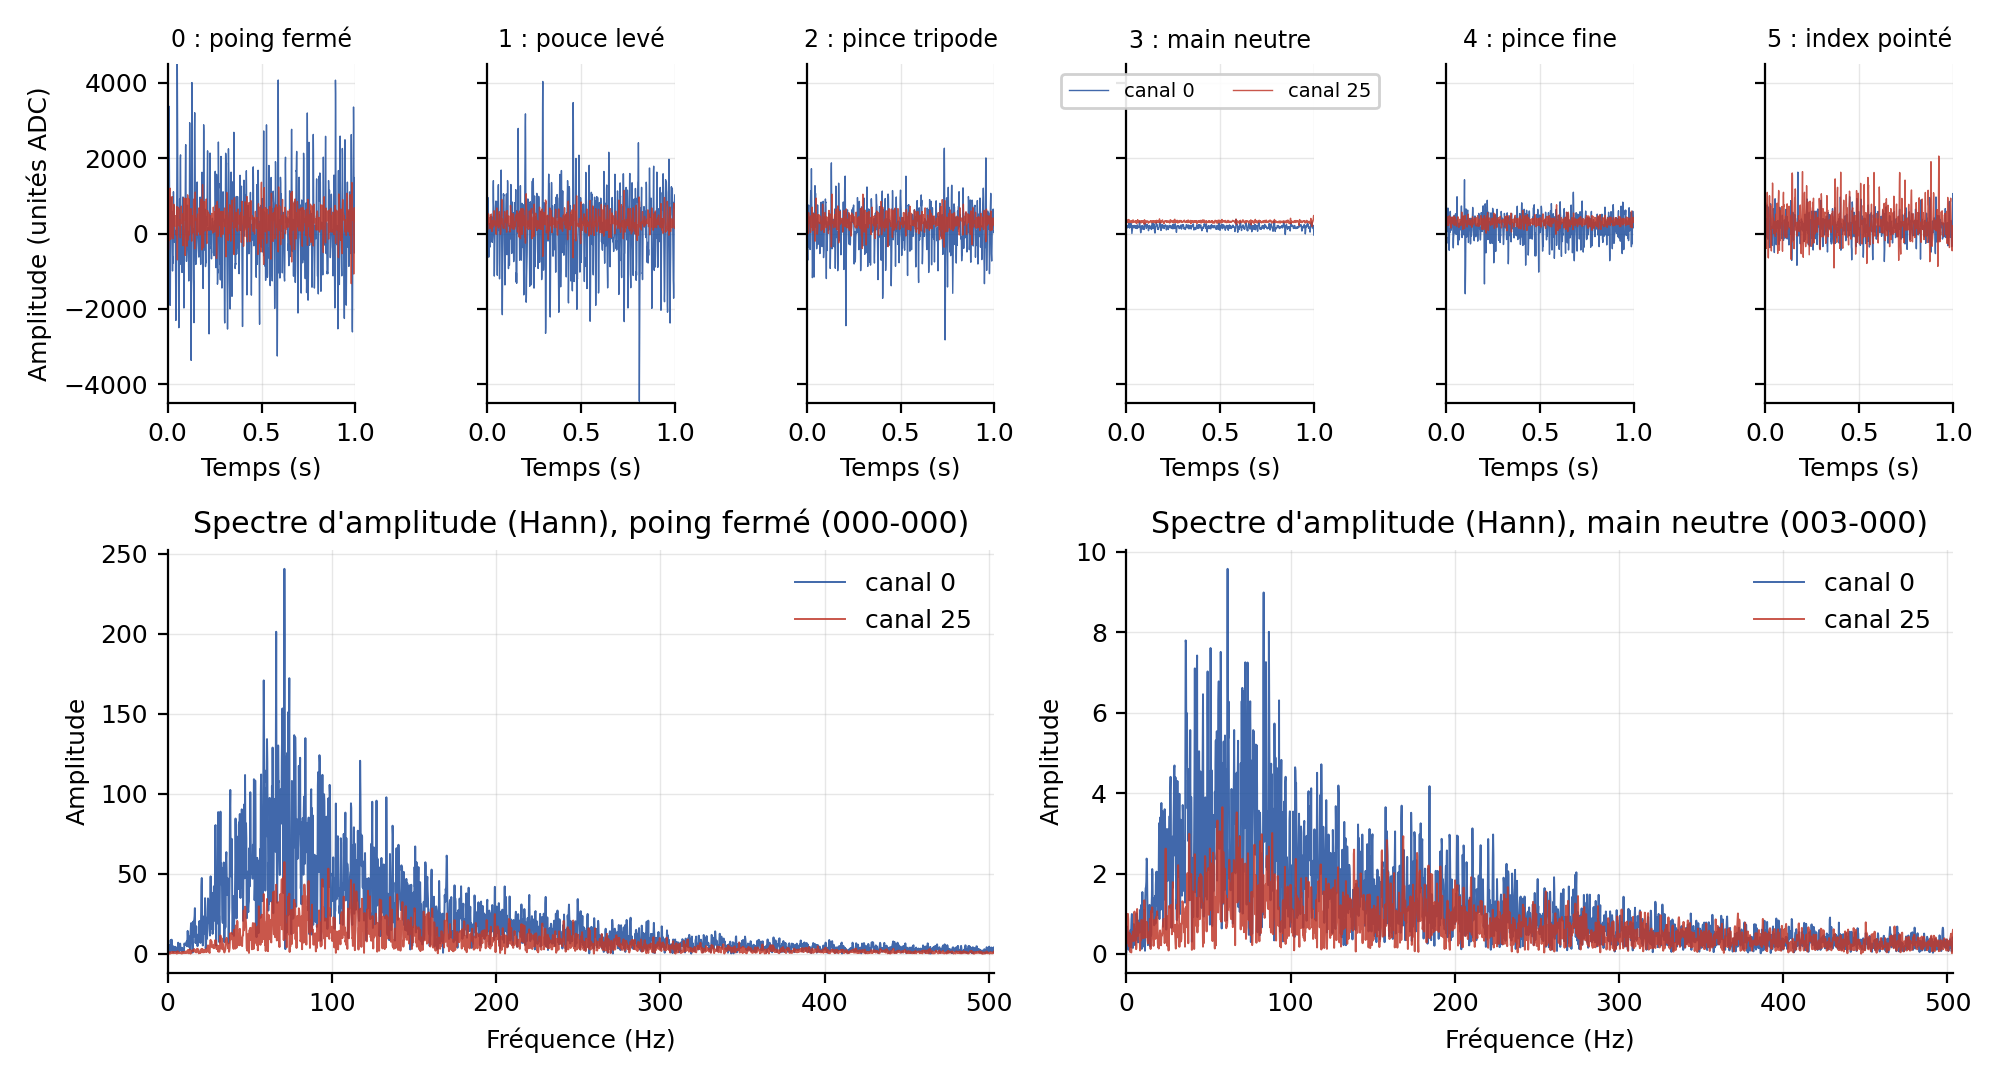
\includegraphics[width=\textwidth]{fig_5_eda.png}
\caption{Haut, 1~s des canaux 0 et 25 pour chacun des six gestes (première répétition); bas, spectres d'amplitude (fenêtre de Hann) du poing fermé (000-000.csv) et de la main neutre (003-000.csv). L'énergie de l'EMG se situe surtout entre 20 et 250~Hz; le canal 25 présente un décalage DC d'environ 300 unités.}
\label{fig:eda}
\end{figure}

\question{5.4 (Question 1)}
Les quatre classificateurs ont d'abord été comparés comme dans le bloc-notes, dans le plan des features 6 et 7 (SD normalisé des canaux 0 et 25) avec un seul tirage 50/50 (Figure~\ref{fig:frontieres}). Comme un seul tirage dépend fortement des fenêtres tombées dans l'ensemble de test, l'évaluation a aussi été répétée par validation croisée (3 plis $\times$ 20 répétitions), en 2D et avec les 12 features (Table~\ref{tab:scores}).

\begin{figure}[H]
\centering
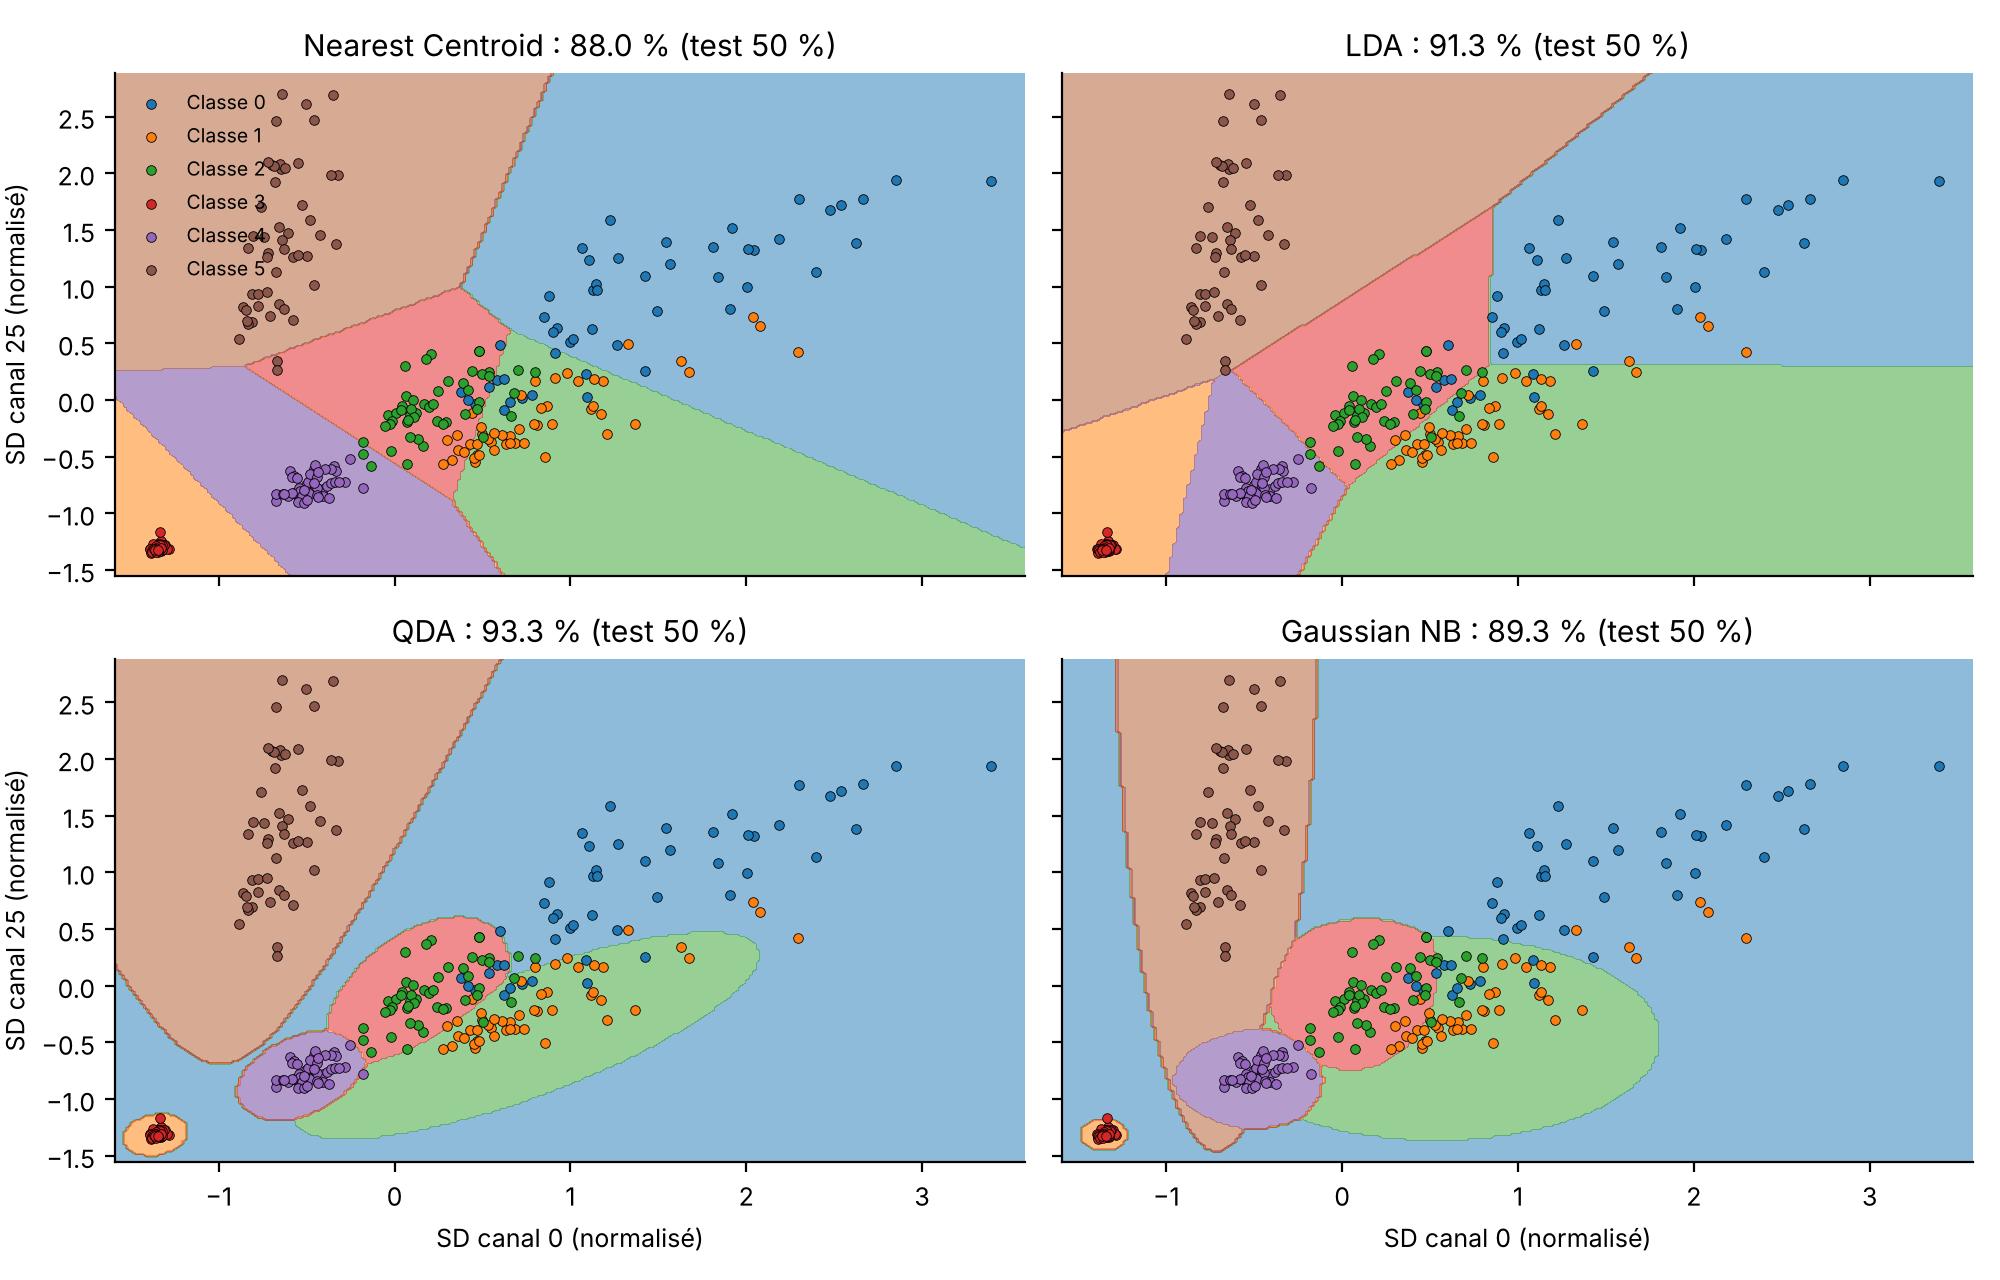
\includegraphics[width=\textwidth]{fig_5_frontieres.png}
\caption{Régions de décision des quatre classificateurs dans le plan (SD canal 0, SD canal 25), entraînés sur 50~\% des 300 fenêtres. Chaque point est une fenêtre de 200 échantillons et sa couleur, le geste réel. Le score indiqué est celui des 50~\% de fenêtres de test.}
\label{fig:frontieres}
\end{figure}

\begin{table}[H]
\centering
\caption{Exactitude des quatre classificateurs. La première colonne reproduit la méthode du bloc-notes (un seul tirage). Les deux autres donnent la moyenne et l'écart-type sur 60 entraînements (validation croisée à 3 plis répétée 20 fois).}
\label{tab:scores}
\begin{tabular}{lccc}
\toprule
Classificateur & 2 features, 1 tirage 50/50 & 2 features, k-fold 3$\times$20 & 12 features, k-fold 3$\times$20\\
\midrule
Nearest Centroid & 88,0~\% & 85,9 $\pm$ 3,3~\% & 88,9 $\pm$ 2,7~\%\\
LDA & 91,3~\% & 90,5 $\pm$ 2,9~\% & \textbf{94,2 $\pm$ 1,9~\%}\\
QDA & \textbf{93,3~\%} & \textbf{90,6 $\pm$ 2,2~\%} & 94,2 $\pm$ 2,2~\%\\
Gaussian NB & 89,3~\% & 87,6 $\pm$ 3,1~\% & 89,9 $\pm$ 2,9~\%\\
\bottomrule
\end{tabular}
\end{table}

La LDA est le classificateur le plus fiable pour ce jeu de données.
\begin{itemize}
\item \textbf{Meilleur score et plus petite dispersion.} Avec 12 features, LDA et QDA sont à égalité (94,2~\%) mais la LDA a le plus petit écart-type entre plis (1,9~\%); en 2D, les deux sont indiscernables (90,5 et 90,6~\%). L'avance de la QDA avec un seul tirage (93,3 contre 91,3~\%) n'était qu'un effet du tirage.
\item \textbf{Les classes sont allongées et corrélées} (Figure~\ref{fig:frontieres}, le SD des canaux 0 et 25 varient ensemble pour les classes 0, 1 et 2). Le Nearest Centroid (distance euclidienne au centre de classe) et le Gaussian NB (covariance diagonale, ellipses alignées sur les axes) ne modélisent pas cette corrélation; la LDA et la QDA utilisent la covariance complète et orientent leurs frontières le long des nuages.
\item \textbf{La LDA a beaucoup moins de paramètres.} Elle estime une seule matrice de covariance partagée (78 paramètres, 200 fenêtres d'entraînement) alors que la QDA en estime une par classe ($6 \times 78 = 468$ paramètres, environ 33 fenêtres par classe). Avec des features presque colinéaires (RMS, Var, SD, MAV), scikit-learn doit même régulariser la covariance de la QDA, qui devient sensible aux fenêtres tirées. Les frontières de la LDA, qui maximisent le critère de Fisher (variance interclasse sur variance intraclasse), sont plus stables.
\item \textbf{Erreurs concentrées sur trois gestes.} Les matrices de confusion (Figure~\ref{fig:confusion}) montrent que les erreurs se limitent au poing fermé (0), au pouce levé (1) et à la pince tripode (2), dont les features se chevauchent; la main neutre, la pince fine et l'index pointé sont reconnus à 97 à 100~\%.
\end{itemize}

\begin{figure}[H]
\centering
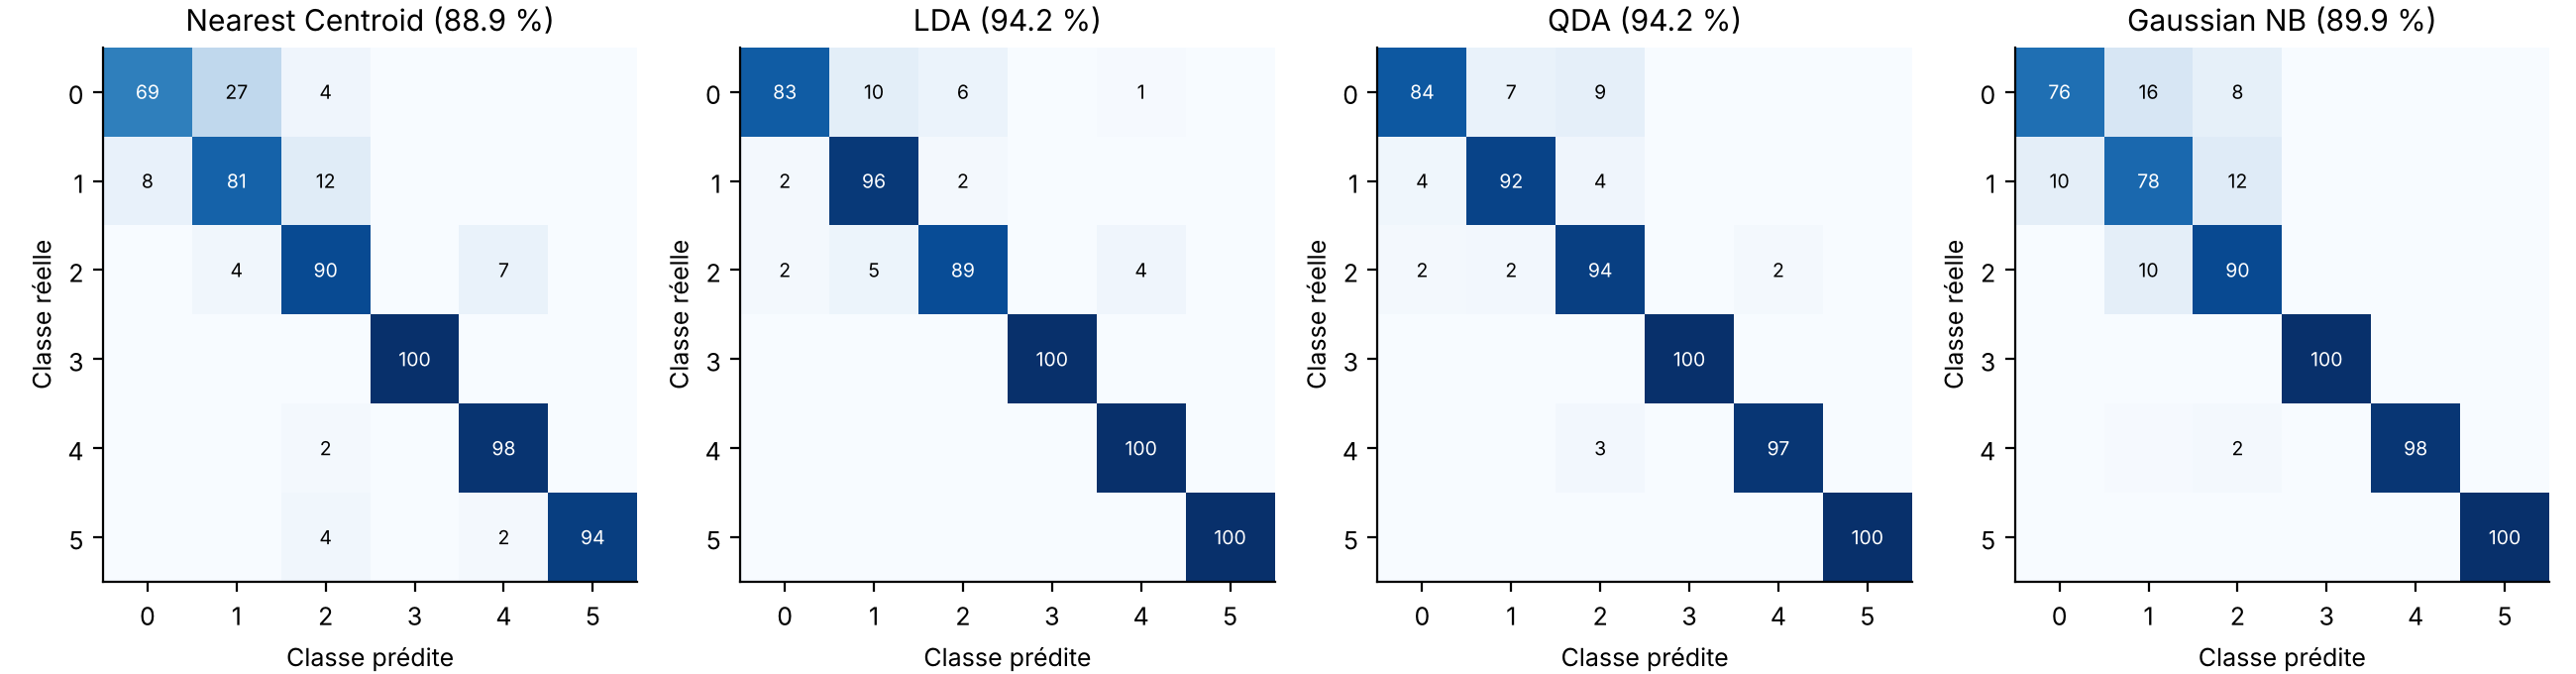
\includegraphics[width=\textwidth]{fig_5_confusion.png}
\caption{Matrices de confusion (en \% des fenêtres de chaque classe réelle) cumulées sur la validation croisée 3$\times$20 avec les 12 features. Le Nearest Centroid classe 27~\% des poings fermés comme des pouces levés.}
\label{fig:confusion}
\end{figure}

\question{5.5 (Question 2)}
Les scores sont ceux de la Table~\ref{tab:scores} et de la Figure~\ref{fig:scores}. Avec la méthode du bloc-notes (deux features SD, un tirage 50/50), nous obtenons 88,0~\% (Nearest Centroid), 91,3~\% (LDA), 93,3~\% (QDA) et 89,3~\% (Gaussian NB); en validation croisée 3$\times$20 avec les 12 features, 88,9~\%, 94,2~\%, 94,2~\% et 89,9~\%. Le score de la LDA calculé exactement comme dans le bloc-notes (\texttt{RepeatedKFold} 3$\times$3, 12 features) est de 94,3~\%, identique à la valeur du bloc-notes fourni. Un seul tirage est peu représentatif, en répétant 100 fois la séparation 50/50, le score du Nearest Centroid varie de 79 à 91~\% et celui de la LDA de 85 à 94~\%.

\begin{figure}[H]
\centering
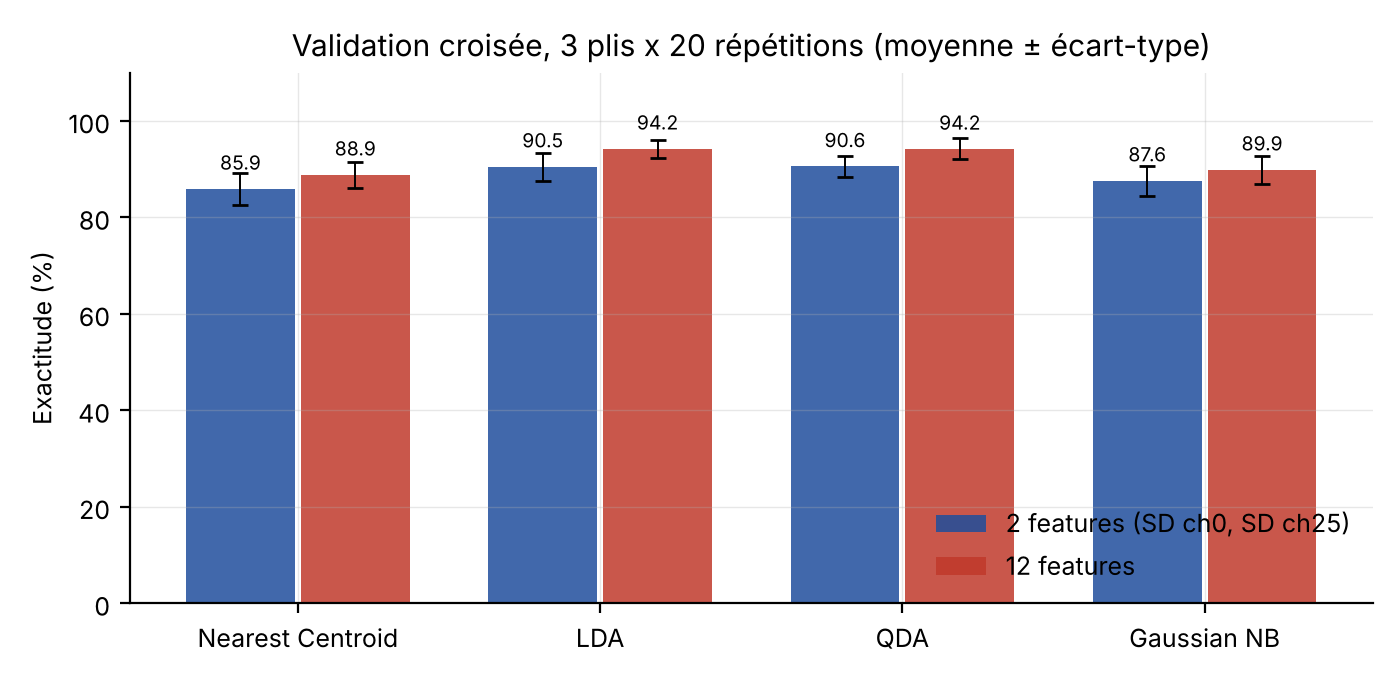
\includegraphics[width=0.75\textwidth]{fig_5_scores.png}
\caption{Exactitude moyenne et écart-type des quatre classificateurs en validation croisée 3$\times$20, dans le plan des deux features SD et avec le vecteur complet de 12 features.}
\label{fig:scores}
\end{figure}

\question{5.6 (Question 3)}
\textbf{Segmentation.} Chaque fichier (environ 5~s) est découpé par \texttt{segment\_dataset} en fenêtres consécutives de 200 échantillons (199~ms à 1007~Hz) sans recouvrement, soit 25 fenêtres par fichier et 300 au total (50 par geste); seuls les canaux 0 et 25 sont retenus et l'étiquette est lue dans le nom du fichier (AAA-BBB.csv, AAA le geste, BBB la répétition). Une fenêtre de 200~ms reste sous le délai d'environ 300~ms acceptable pour commander une prothèse en temps réel.

\textbf{Quantification.} \texttt{features\_dataset} résume chaque fenêtre de $N = 200$ échantillons $x[i]$ par six features temporelles par canal, la valeur absolue moyenne (MAV), la valeur efficace (RMS), la « variance » (Var), l'écart-type (SD), les passages par zéro (ZC) et les changements de signe de la pente (SSC) :
\begin{align*}
\text{MAV} &= \tfrac{1}{N}\textstyle\sum_i |x[i]|, & \text{RMS} &= \sqrt{\tfrac{1}{N}\textstyle\sum_i x[i]^2},\\
\text{Var} &= \tfrac{1}{N-1}\textstyle\sum_i x[i]^2, & \text{SD} &= \sqrt{\tfrac{1}{N-1}\textstyle\sum_i (x[i]-\bar{x})^2},\\
\text{ZC} &= \#\{\,x[i]\,x[i+1] < 0\,\}, & \text{SSC} &= \#\{\,(x[i]-x[i-1])(x[i]-x[i+1]) > 0\,\},
\end{align*}
où la « variance » du bloc-notes est en fait une somme des carrés sans retrait de la moyenne. Les 6 valeurs de chaque canal sont concaténées en un vecteur $\mathbf{x} \in \mathbb{R}^{12}$ par fenêtre, $\mathbf{x} = [\text{MAV}_0,$ $\text{MAV}_{25},$ $\text{RMS}_0,$ $\text{RMS}_{25},$ $\ldots,$ $\text{SSC}_0,$ $\text{SSC}_{25}]$, comme dans la figure de la section 2 du bloc-notes. La matrice $300 \times 12$ est ensuite normalisée colonne par colonne (\texttt{preprocessing.scale}, moyenne nulle, écart-type unitaire) pour que des features d'échelles très différentes (Var en unités au carré, ZC en nombre d'événements) aient le même poids. La Figure~\ref{fig:boxplot} montre la distribution des 12 features par geste, les quatre features d'amplitude sont très redondantes, le canal 25 sépare bien l'index pointé (5) que le canal 0 confond avec la pince fine, et les ZC du canal 0 isolent la main neutre.

\begin{figure}[H]
\centering
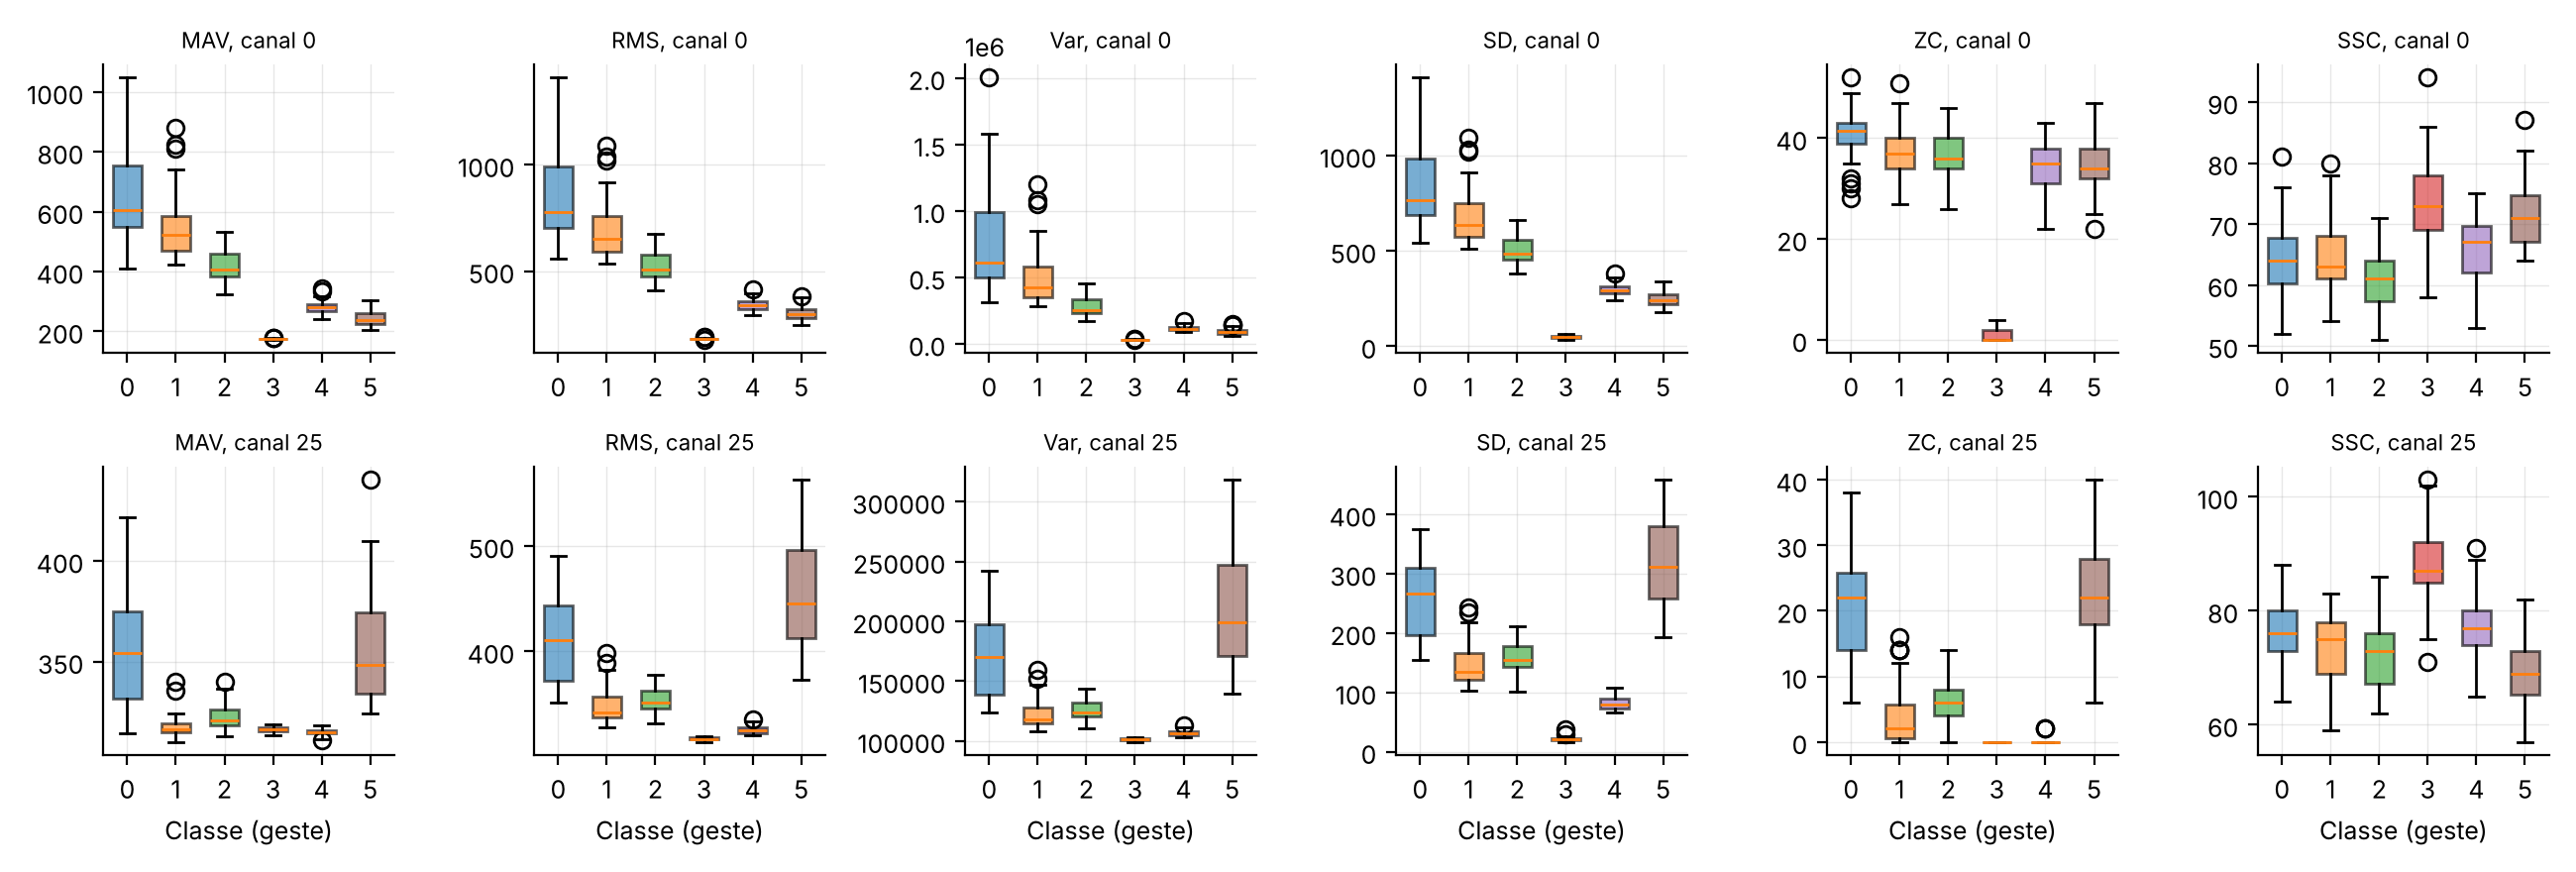
\includegraphics[width=\textwidth]{fig_5_features_boxplot.png}
\caption{Distribution des 12 features (avant normalisation) selon le geste, sur les 50 fenêtres de chaque classe. Haut, canal 0; bas, canal 25.}
\label{fig:boxplot}
\end{figure}

\textbf{Un point de la figure de classification} (Figure~\ref{fig:frontieres}) est donc une fenêtre de 200 échantillons (199~ms) d'EMG, placée selon le SD normalisé du canal 0 (indice 6, abscisse) et du canal 25 (indice 7, ordonnée). Sa couleur est le geste lu dans le nom du fichier; les régions colorées sont la décision du classificateur pour tout nouveau point.

\question{5.7 (Question 4)}
La division sert à mesurer la capacité de généralisation, c'est-à-dire l'exactitude sur des fenêtres jamais vues, ce qui est la situation réelle d'une prothèse. Évalué sur ses propres fenêtres d'entraînement, un modèle obtient un score optimiste qui cache le surapprentissage (mémorisation du bruit et des artefacts plutôt que des caractéristiques du geste), surtout pour la QDA, qui a beaucoup de paramètres par rapport au nombre de fenêtres. Dans le bloc-notes, \texttt{train\_test\_split} sépare 50~\% des fenêtres pour tracer les frontières et \texttt{RepeatedKFold} forme les plis du score de la LDA; dans les deux cas, \texttt{fit} ne voit que l'ensemble d'apprentissage et \texttt{score} que l'ensemble de test.

\question{5.8 (Question 5)}
La validation croisée k-fold répétée (\texttt{RepeatedKFold}, 3 plis $\times$ 3 répétitions dans le bloc-notes). Le jeu de données est divisé en 3 plis; chacun sert tour à tour d'ensemble de test pendant que les deux autres (2/3 des fenêtres) servent à l'entraînement, puis l'opération est reprise avec de nouveaux découpages, soit 9 entraînements dont on moyenne les scores. Chaque fenêtre est testée exactement une fois par répétition, aucune n'est gaspillée, et la moyenne réduit la variance due au tirage, qui atteint une dizaine de points avec un seul tirage (question 2). Avec 3 plis $\times$ 20 répétitions, l'écart-type entre plis est de 2 à 3~\% (Table~\ref{tab:scores}), ce qui quantifie l'incertitude sur le score moyen.

\section*{6. Exemple d'application pour la prédiction de l'effort ECG}

Le jeu de données compte six fichiers, un par niveau d'effort (0 à 100~\% par pas de 20~\%), de 56 à 104~s, échantillonnés à 2000~Hz sur l'entrée ADC0 (volts, ligne de base vers 1,75~V). Comme dans le bloc-notes, chaque fichier est découpé en fenêtres de 20\,000 échantillons (10~s) avec un recouvrement de 50~\%, soit 79 fenêtres (19, 14, 13, 10, 13 et 10 par niveau). Deux modifications ont été apportées à la classe \texttt{QRSDetectorOffline}, ce que l'énoncé permet.
\begin{itemize}
\item Ses paramètres en échantillons (fenêtre d'intégration 120, espacement minimal 100, période réfractaire 200) sont prévus pour 1~kHz (« change proportionally when adjusting frequency »); nous les avons doublés pour 2~kHz, ce qui ramène la période réfractaire à 200~ms comme chez Pan-Tompkins. À 80~\% d'effort, la proportion d'intervalles RR aberrants passe de 23 à 15~\%.
\item La formule \texttt{int(len/L*2)} produisait une dernière fenêtre tronquée (par exemple 10\,198 points sur 20\,000 pour 020-000.csv), qui faussait les features; seules les fenêtres complètes sont gardées.
\end{itemize}

\question{6.3 (Exercice 1.0)}
La Figure~\ref{fig:detection} montre les étapes du détecteur de Pan-Tompkins sur le fichier 000-000.csv (repos).
\begin{itemize}
\item \textbf{Filtre passe-bande} Butterworth d'ordre 4, de 5 à 25~Hz, qui élimine la dérive de la ligne de base, l'interférence à 60~Hz et le bruit haute fréquence.
\item \textbf{Dérivée, puis élévation au carré}, qui mettent en évidence la pente raide du complexe QRS et rendent le signal positif.
\item \textbf{Intégration à fenêtre glissante} (240 échantillons, 120~ms), qui produit une bosse par battement.
\item \textbf{Seuillage adaptatif}, qui repère le maximum de chaque bosse (points noirs).
\end{itemize}
Les indices retournés sont ceux du signal intégré; le filtre étant causal et l'intégration s'étendant sur 240 échantillons, ils sont en retard de 90 à 110~ms sur l'onde R (dernier panneau). Pour nos features, l'onde R est retrouvée au maximum du signal brut dans les 175~ms qui précèdent chaque indice.

\begin{figure}[H]
\centering
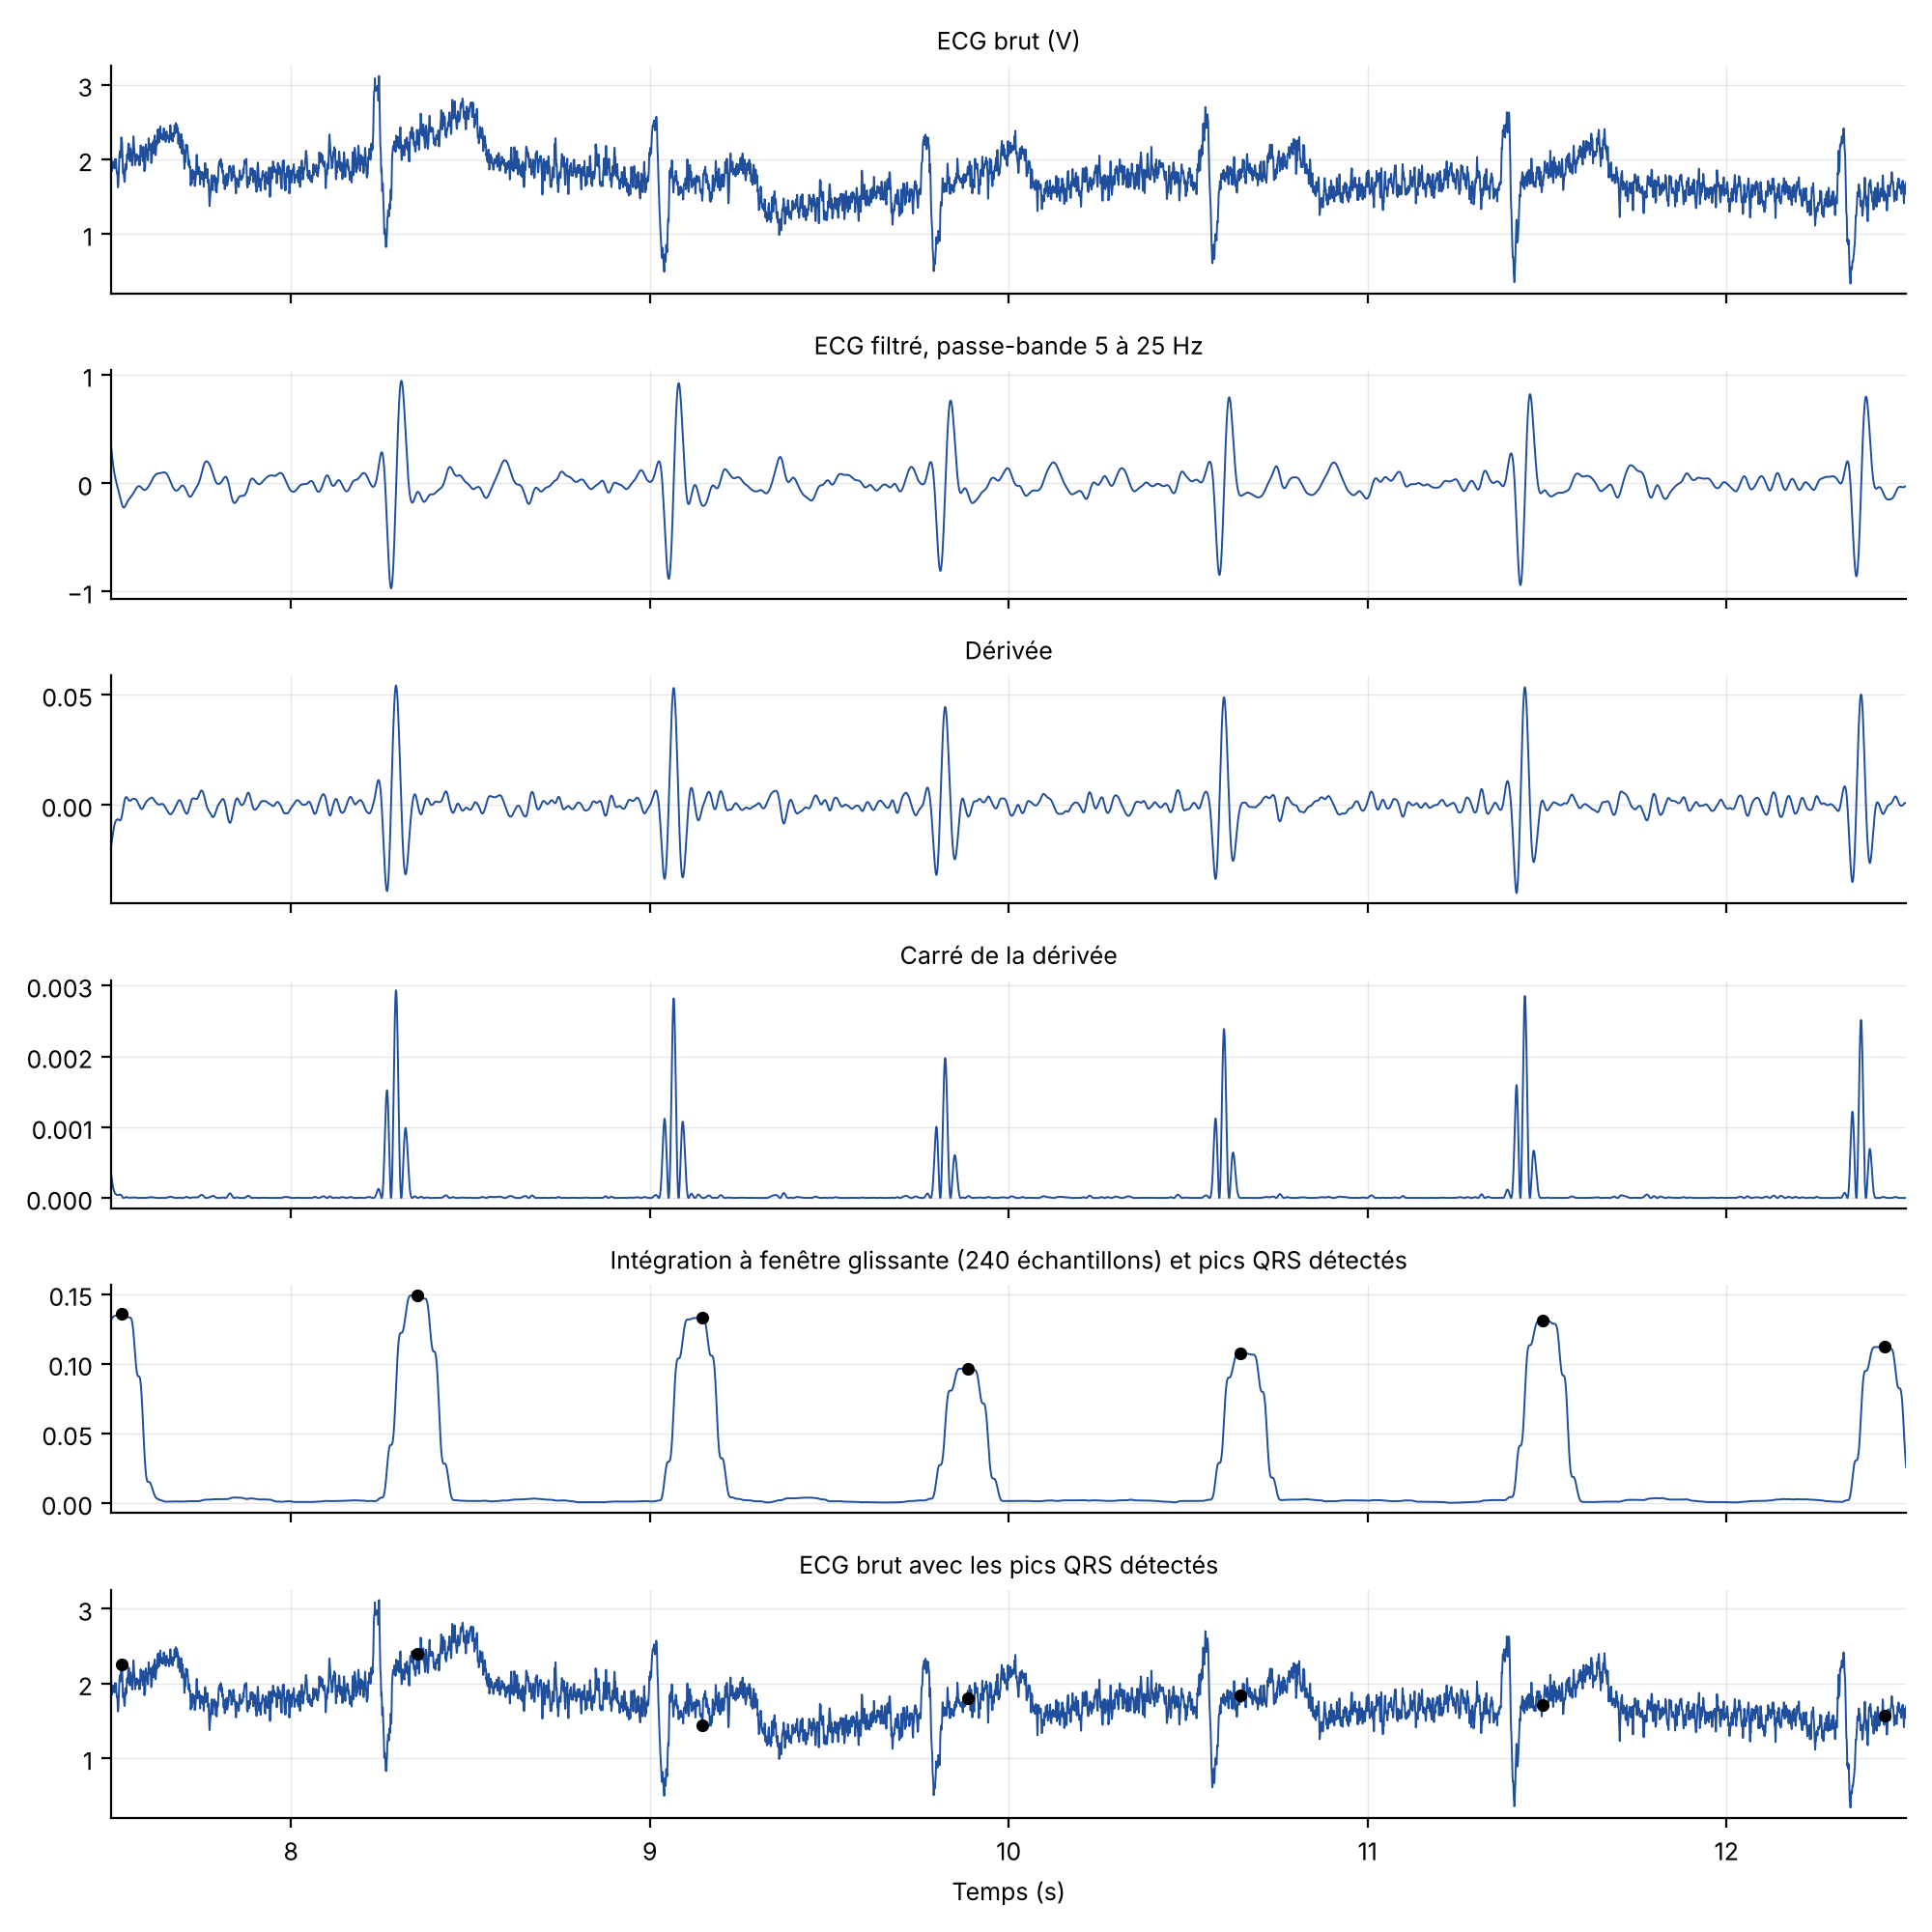
\includegraphics[width=0.78\textwidth]{fig_6_1_detection.png}
\caption{Étapes de l'algorithme de Pan-Tompkins sur 5~s du fichier 000-000.csv (effort 0~\%). De haut en bas, ECG brut, filtré, dérivé, élevé au carré, intégré avec les pics QRS détectés, puis ECG brut avec les mêmes indices, qui tombent environ 100~ms après l'onde R.}
\label{fig:detection}
\end{figure}

La Figure~\ref{fig:niveaux} montre 5~s de chaque niveau. La fréquence cardiaque monte de 70 à environ 157~bpm, et le signal se dégrade nettement à partir de 60~\% (bruit musculaire et artefacts de mouvement d'amplitude comparable au QRS). La proportion d'intervalles RR aberrants (plus court que 0,7 fois ou plus long que 1,4 fois la médiane, donc fausses détections ou battements manqués) est nulle à 0 et 20~\%, puis de 5, 8, 15 et 13~\% à 40, 60, 80 et 100~\%.

\begin{figure}[H]
\centering
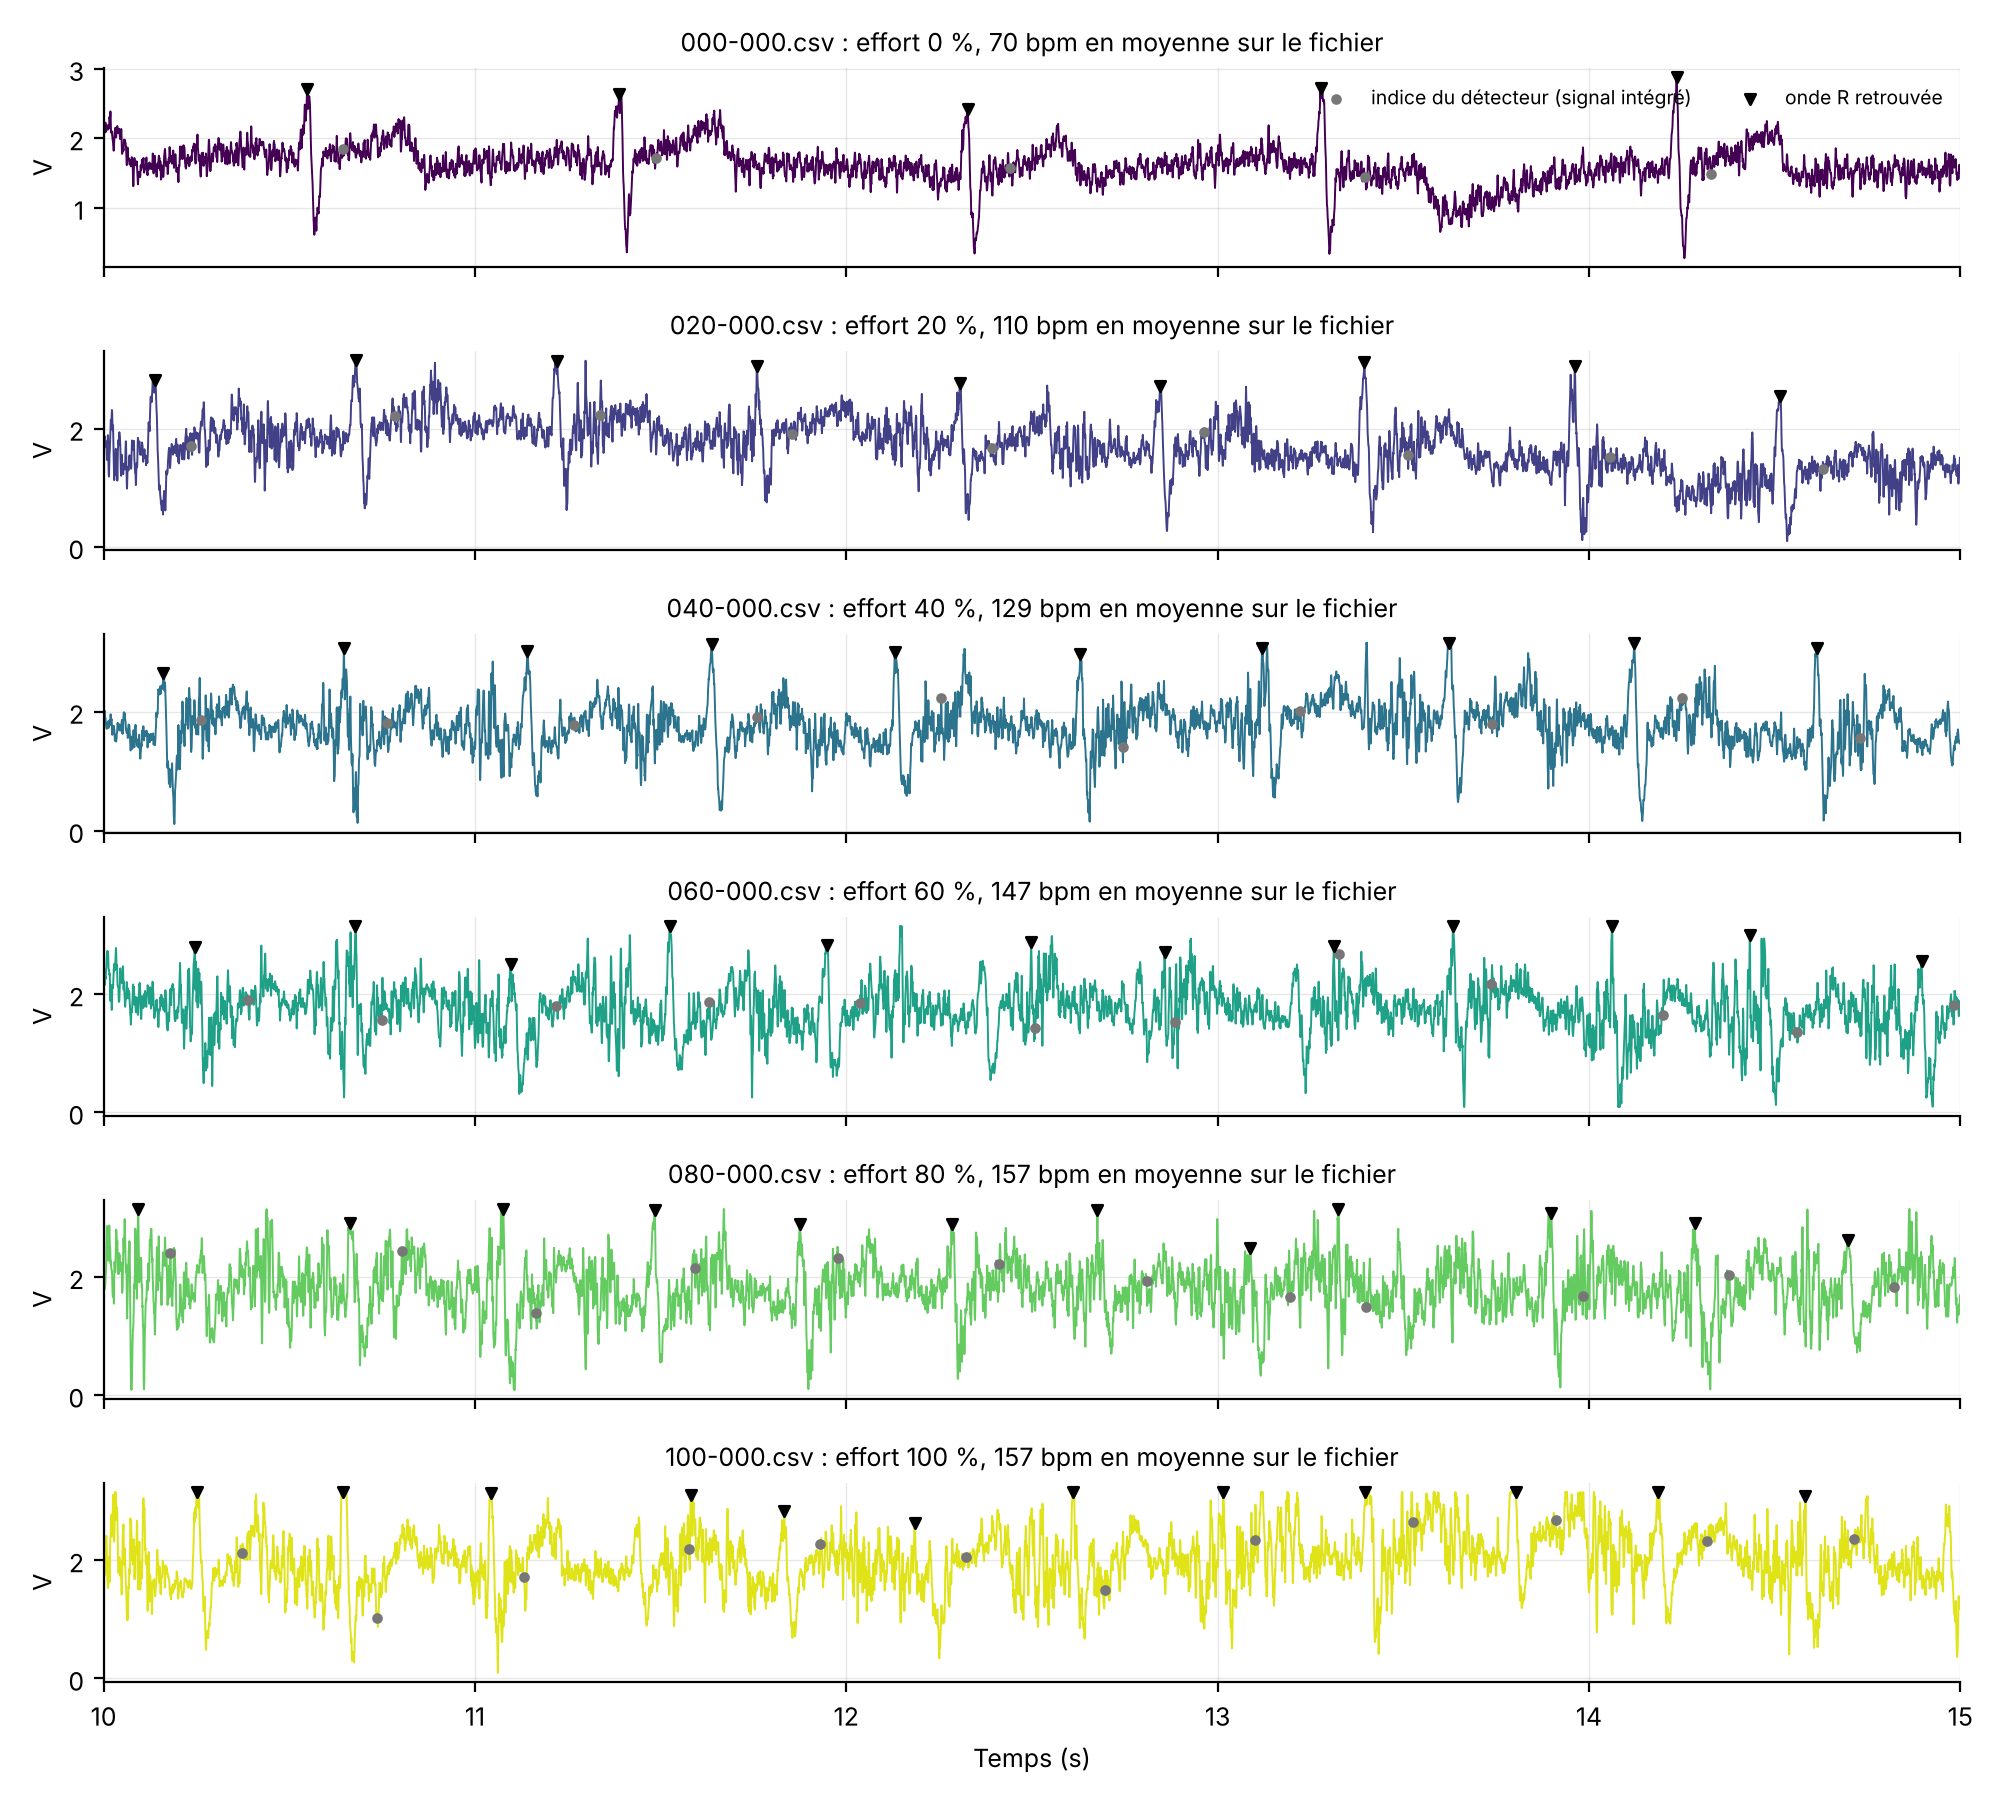
\includegraphics[width=\textwidth]{fig_6_1_niveaux.png}
\caption{Cinq secondes d'ECG brut (de 10 à 15~s) pour chaque niveau d'effort. Les points gris sont les indices retournés par le détecteur et les triangles noirs les ondes R retrouvées. La fréquence cardiaque indiquée est la moyenne sur le fichier.}
\label{fig:niveaux}
\end{figure}

\question{6.4 (Exercice 2.0, GEL-7072 : 4 features minimum)}
Cinq features sont calculées par fenêtre de 10~s, à partir des positions des ondes R et du signal brut de la fenêtre (Table~\ref{tab:features}, Figure~\ref{fig:features}).

\begin{table}[H]
\centering
\caption{Features calculées sur chaque fenêtre de 10~s et leur moyenne pour chaque niveau d'effort.}
\label{tab:features}
\small
\begin{tabular}{llcccccc}
\toprule
Feature & Calcul & 0~\% & 20~\% & 40~\% & 60~\% & 80~\% & 100~\%\\
\midrule
Fréquence cardiaque (bpm) & $60\,000 / \text{médiane}(RR)$ & 70,5 & 110,3 & 126,3 & 145,4 & 155,5 & 157,8\\
SDNN (ms) & écart-type des RR & 44,6 & 14,6 & 46,6 & 81,2 & 89,7 & 79,4\\
RMSSD (ms) & $\sqrt{\text{moy}(\Delta RR^2)}$ & 32,2 & 20,8 & 51,5 & 116,8 & 127,0 & 115,6\\
Amplitude de l'onde R (V) & médiane de $x[R] - \text{médiane}(x)$ & 1,06 & 1,21 & 1,20 & 1,11 & 1,19 & 1,12\\
Écart-type du signal (V) & $\sigma$ du signal brut & 0,31 & 0,42 & 0,43 & 0,44 & 0,47 & 0,49\\
\bottomrule
\end{tabular}
\end{table}

\begin{itemize}
\item \textbf{Fréquence cardiaque.} Réponse physiologique la plus directe à l'effort (le débit cardiaque suit la demande en oxygène des muscles). Calculée à partir de la médiane des intervalles RR plutôt qu'en comptant les pics comme dans le bloc-notes, pour être insensible aux pics manqués ou en trop aux efforts élevés.
\item \textbf{SDNN et RMSSD.} Mesures classiques de la variabilité cardiaque dans le domaine temporel, l'écart-type des RR et la racine de la moyenne des carrés des différences entre RR successifs (plus sensible battement à battement). La variabilité diminue normalement avec l'effort par retrait du tonus vagal.
\item \textbf{Amplitude de l'onde R.} Médiane de $x[R]$ moins la médiane de la fenêtre (ligne de base). Hypothèse, la respiration plus ample, les mouvements du thorax et la sudation (impédance de contact plus faible) modifient l'amplitude du QRS.
\item \textbf{Écart-type du signal brut.} Énergie totale de la fenêtre, donc le QRS plus le bruit électromyographique (muscles pectoraux et abdominaux, respiration profonde) et les artefacts de mouvement, qui augmentent avec l'effort.
\end{itemize}

\begin{figure}[H]
\centering
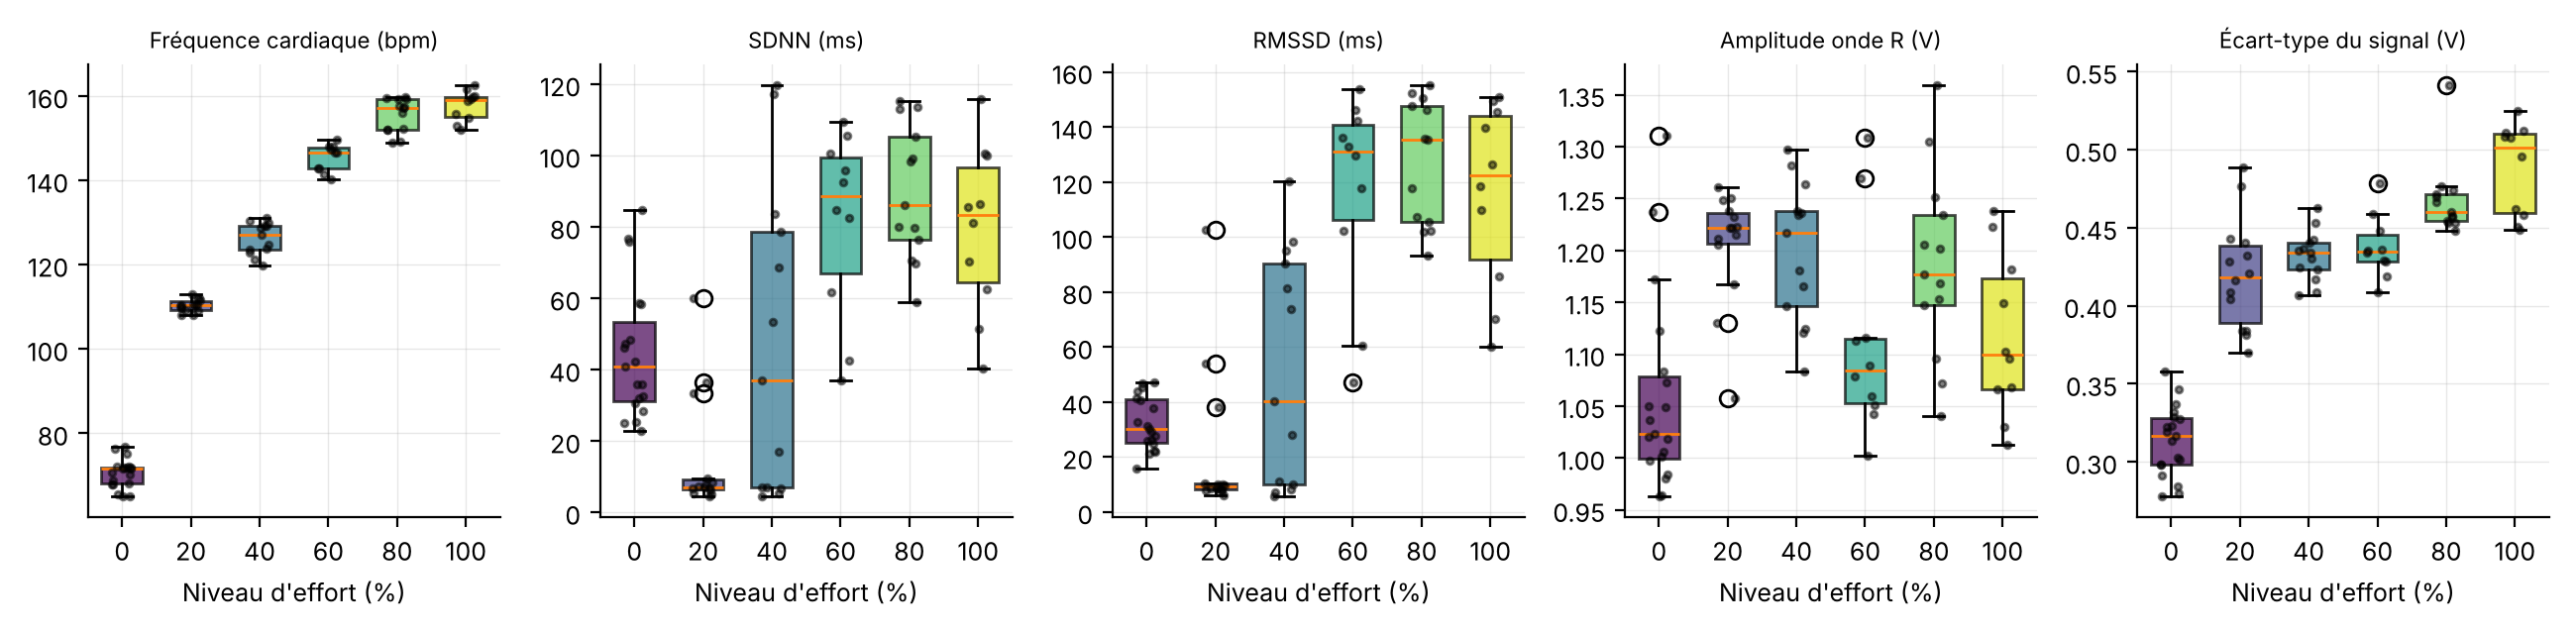
\includegraphics[width=\textwidth]{fig_6_2_features.png}
\caption{Distribution des cinq features par niveau d'effort (une boîte par niveau, un point par fenêtre de 10~s).}
\label{fig:features}
\end{figure}

La fréquence cardiaque croît de façon monotone et presque sans chevauchement jusqu'à 80~\%, puis plafonne (155 et 158~bpm à 80 et 100~\%); l'écart-type du signal croît aussi, avec un chevauchement entre 20 et 60~\%; l'amplitude de l'onde R ne montre aucune tendance. Les deux mesures de variabilité augmentent avec l'effort, à l'inverse de la physiologie, parce qu'à partir de 40~\% elles sont dominées par les erreurs de détection (Figure~\ref{fig:tacho}), une fausse détection crée deux intervalles très courts et un battement manqué un intervalle double, ce qui gonfle l'écart-type bien plus que la variabilité sinusale de quelques dizaines de millisecondes. Ces deux features mesurent donc surtout la qualité de la détection, corrélée à l'effort mais pour la mauvaise raison.

\begin{figure}[H]
\centering
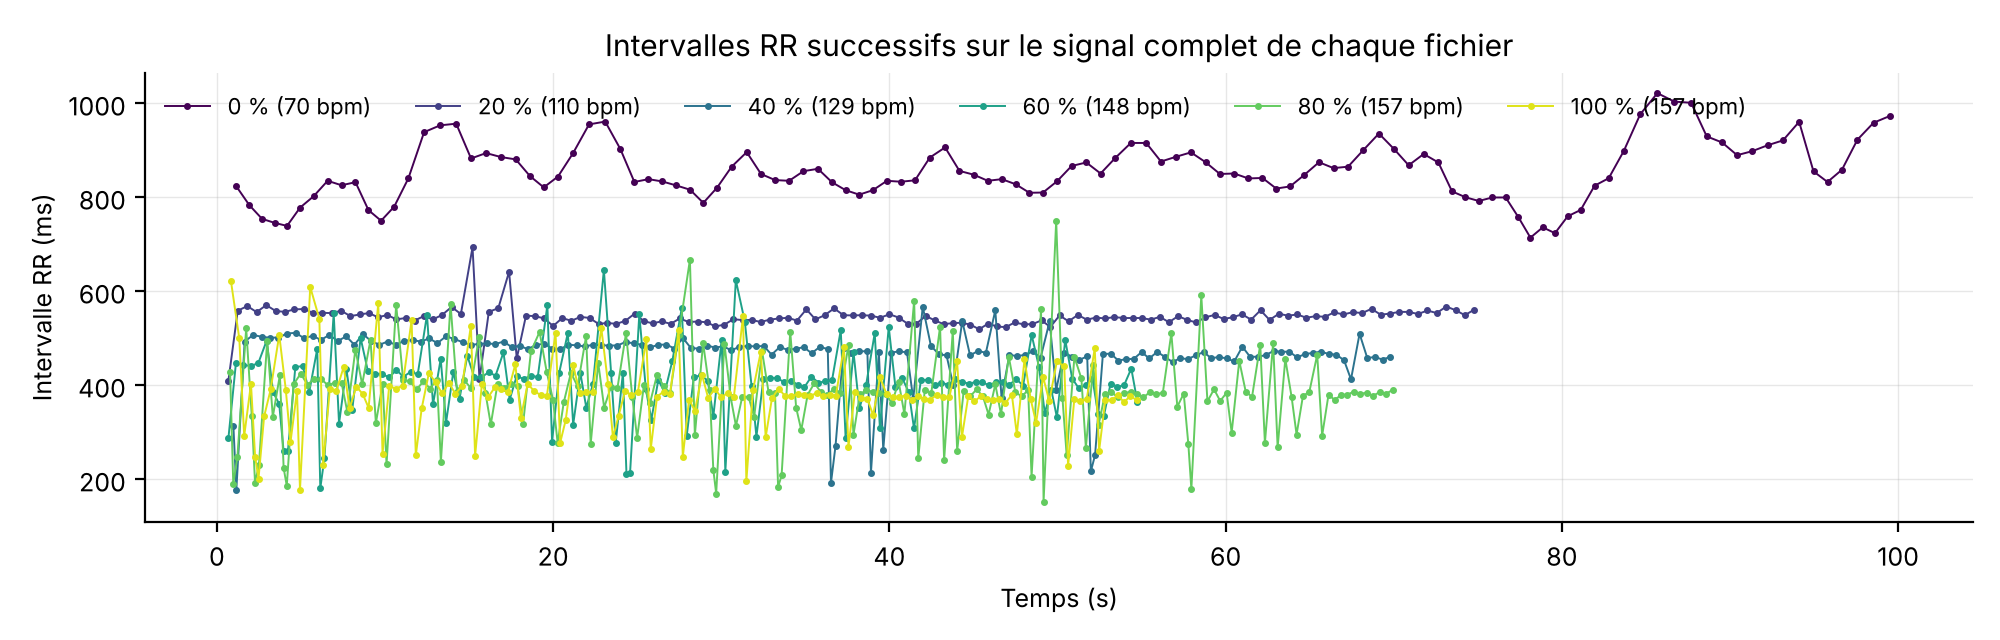
\includegraphics[width=\textwidth]{fig_6_2_tachogramme.png}
\caption{Intervalles RR successifs sur l'enregistrement complet de chaque niveau. Au repos et à 20~\%, la variabilité est régulière (respiration). Aux niveaux supérieurs, les valeurs isolées à 200~ms ou à 800~ms sont des fausses détections et des battements manqués qui dominent le SDNN et le RMSSD.}
\label{fig:tacho}
\end{figure}

\question{6.5 (Exercice 3.0)}
Une LDA entraînée sur les cinq features et évaluée par validation croisée 3 plis $\times$ 3 répétitions, comme dans le module EMG, obtient \textbf{92,9~\%} (91,7 $\pm$ 4,9~\% avec 20 répétitions). La matrice de confusion (Figure~\ref{fig:confecg}) montre que les niveaux 0 à 60~\% sont reconnus à 99 ou 100~\%, alors que 80 et 100~\% se confondent (80~\% reconnu dans 80~\% des cas, 100~\% dans 62~\% seulement), conformément au plateau de la fréquence cardiaque. En retirant une feature à la fois, l'exactitude tombe à 65,7~\% sans la fréquence cardiaque et à 85,4~\% sans l'écart-type du signal, mais reste à 88 à 93~\% sans le SDNN, le RMSSD ou l'amplitude R; la fréquence cardiaque seule donne 84,8~\%.

Comme deux fenêtres voisines partagent 5~s de signal (recouvrement de 50~\%), l'une peut être en apprentissage et l'autre en test, ce qui avantage légèrement le classificateur. En coupant chaque fichier en trois blocs contigus et en testant sur le bloc non vu, l'exactitude reste de 89,3~\%; le résultat n'est donc pas un artefact du recouvrement.

\begin{figure}[H]
\centering
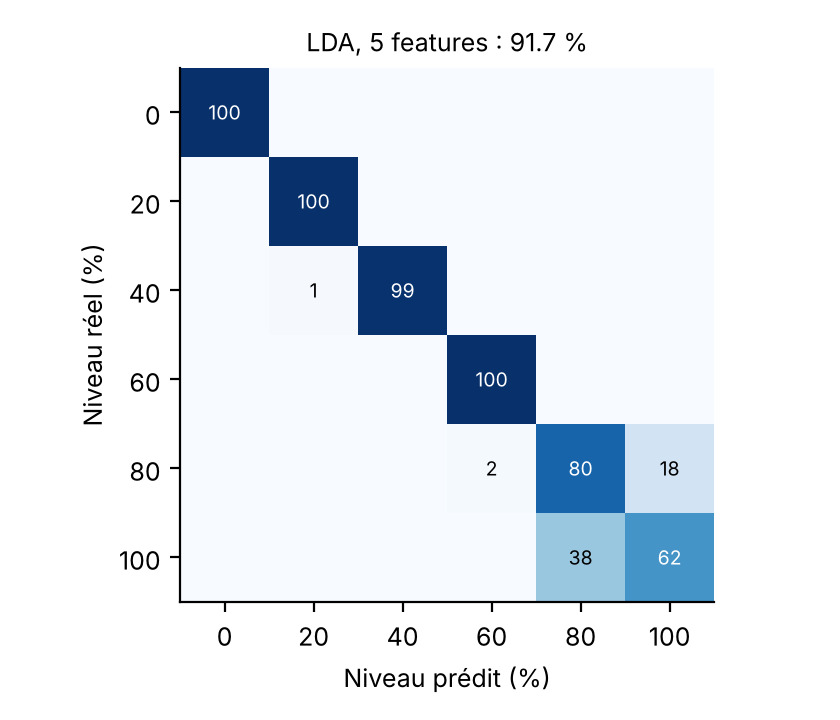
\includegraphics[width=0.45\textwidth]{fig_6_3_confusion.png}
\caption{Matrice de confusion de la LDA avec les cinq features (en \% des fenêtres de chaque niveau réel), cumulée sur la validation croisée 3$\times$20.}
\label{fig:confecg}
\end{figure}

\question{6.6 (Exercice 4.0)}
{\sloppy Pour chaque feature, une régression linéaire simple $\text{effort} = a \cdot \text{feature} + b$ est ajustée sur les 79 fenêtres (\texttt{LinearRegression}) et l'erreur absolue moyenne (MAE) est calculée avec \texttt{metrics.mean\_absolute\_error}. La Figure~\ref{fig:regression} trace les points et la droite, la Table~\ref{tab:mae} résume les erreurs, avec la MAE en validation croisée à 5 plis et le coefficient de corrélation.\par}

\begin{figure}[H]
\centering
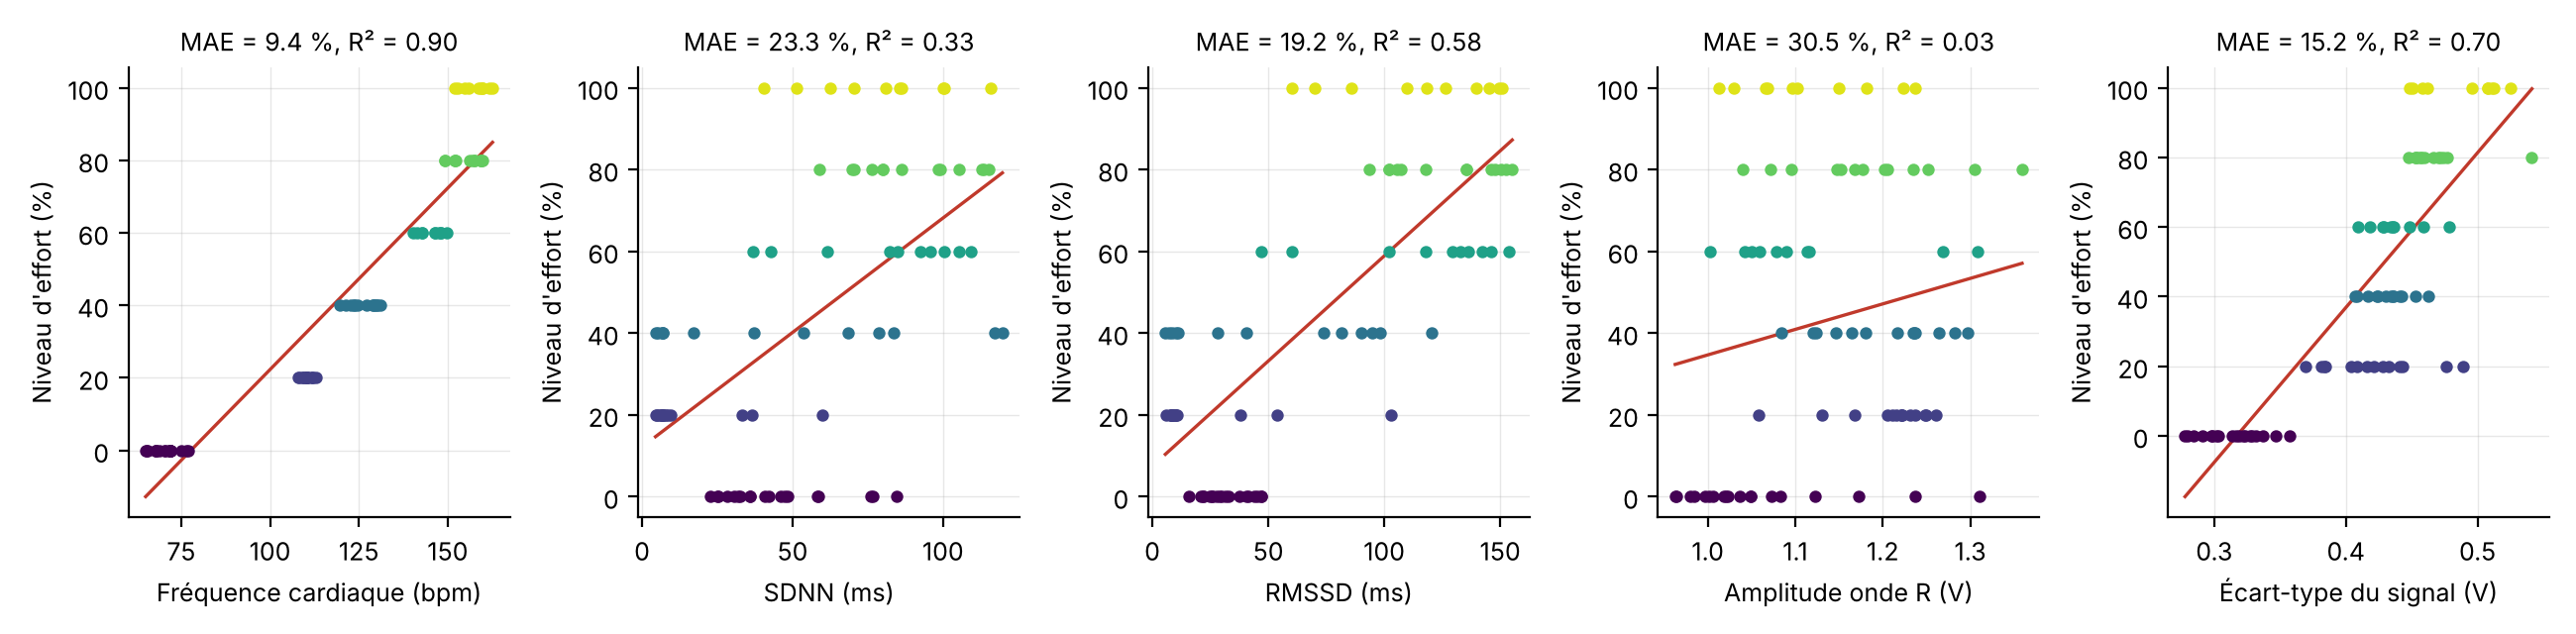
\includegraphics[width=\textwidth]{fig_6_4_regression.png}
\caption{Régression linéaire du niveau d'effort en fonction de chaque feature. Chaque point est une fenêtre de 10~s, coloré selon son niveau réel; la droite rouge est l'ajustement aux moindres carrés.}
\label{fig:regression}
\end{figure}

\begin{table}[H]
\centering
\caption{Performance de la régression linéaire pour chaque feature. La MAE est en points de pourcentage d'effort. Prédire toujours la moyenne des étiquettes donnerait une MAE d'environ 30~\%.}
\label{tab:mae}
\begin{tabular}{lcccc}
\toprule
Feature & MAE (ajustement) & MAE (valid. croisée 5 plis) & $R^2$ & $r$ de Pearson\\
\midrule
Fréquence cardiaque & \textbf{9,4~\%} & 9,7~\% & 0,90 & +0,95\\
Écart-type du signal & 15,2~\% & 15,5~\% & 0,70 & +0,84\\
RMSSD & 19,2~\% & 19,6~\% & 0,58 & +0,76\\
SDNN & 23,3~\% & 24,0~\% & 0,33 & +0,58\\
Amplitude de l'onde R & 30,5~\% & 31,6~\% & 0,03 & +0,18\\
\midrule
Les cinq features ensemble & 7,7~\% & 8,6~\% & 0,93 & \\
\bottomrule
\end{tabular}
\end{table}

La fréquence cardiaque est de loin la feature la plus utile (MAE de 9,4~\%, $R^2$ de 0,90), soit une erreur inférieure au pas de 20~\% entre niveaux; sa relation avec l'effort est presque linéaire jusqu'à 80~\% et le plateau de 80 à 100~\% est la principale source d'erreur. L'écart-type du signal vient en second (15,2~\%). Le RMSSD et le SDNN (19 à 23~\%) ont une relation positive qui reflète la dégradation de la détection plutôt que la physiologie (exercice 2.0). L'amplitude de l'onde R est inutile, sa MAE de 30,5~\% ne vaut pas mieux qu'un prédicteur constant et sa corrélation est nulle. La régression multiple sur les cinq features n'améliore que modestement la fréquence cardiaque seule (7,7 contre 9,4~\%), les autres features apportant peu d'information indépendante.

\question{6.7 (Exercice 5.0)}
Le code fourni a été étendu aux 10 paires possibles de nos 5 features. Pour chaque paire, une LDA entraînée sur 60~\% des fenêtres trace les régions de décision (Figure~\ref{fig:paires}) et son exactitude est aussi mesurée par validation croisée 3$\times$20 (Table~\ref{tab:paires}).

\begin{figure}[H]
\centering
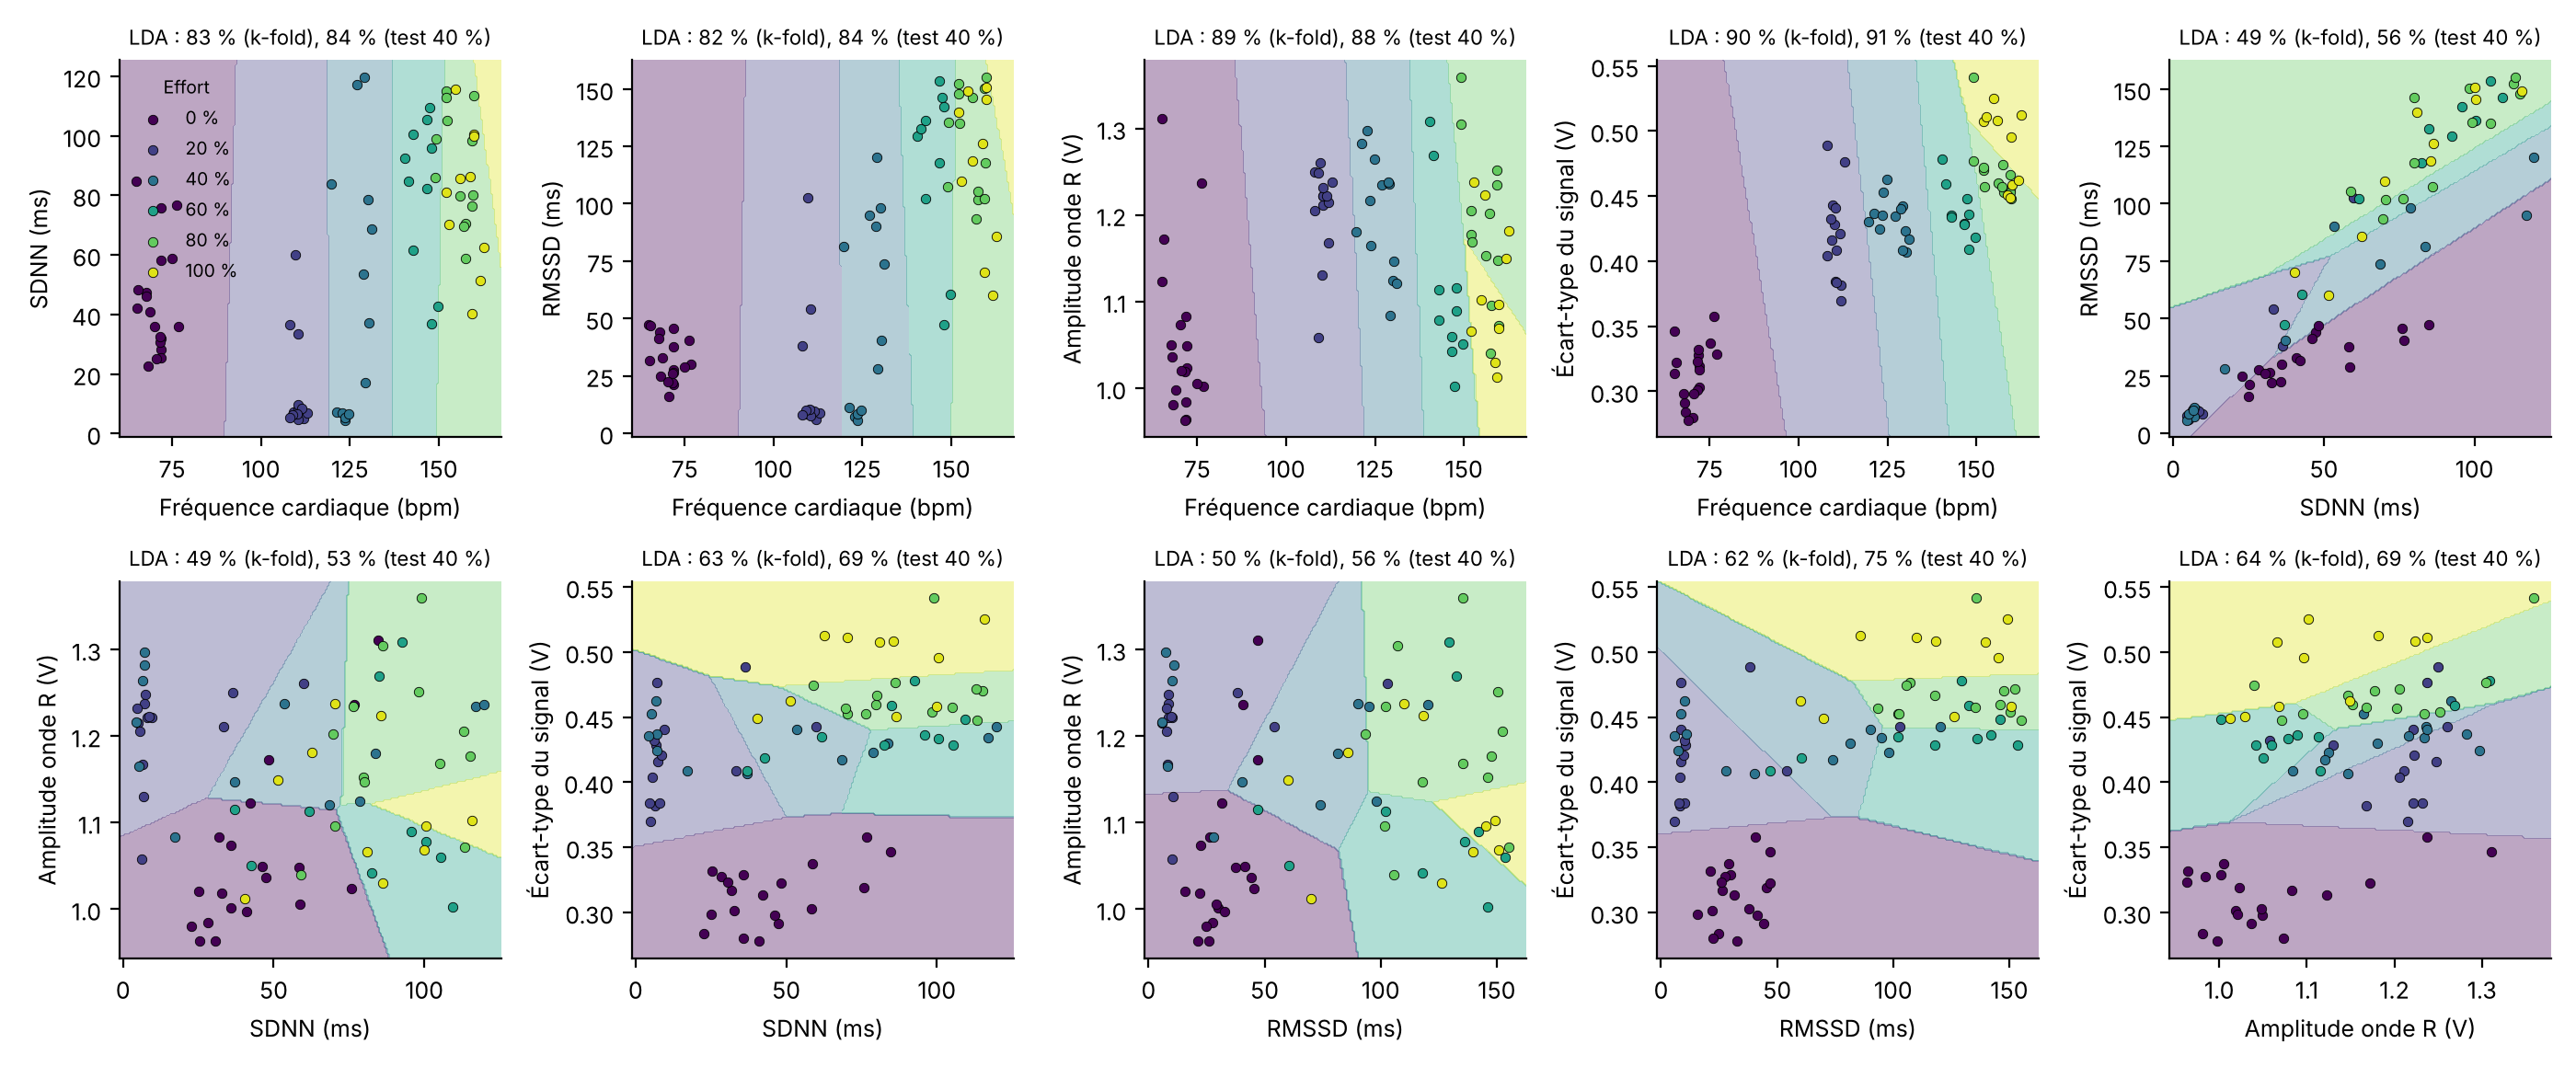
\includegraphics[width=\textwidth]{fig_6_5_paires.png}
\caption{Classification LDA du niveau d'effort pour chaque paire de features. Les régions colorées sont les décisions du classificateur entraîné sur 60~\% des fenêtres, les points sont toutes les fenêtres colorées selon leur niveau réel. Les scores indiqués sont celui de la validation croisée et celui des 40~\% de fenêtres de test.}
\label{fig:paires}
\end{figure}

\begin{table}[H]
\centering
\caption{Exactitude de la LDA pour chaque paire de features (validation croisée 3$\times$20, puis tirage 60/40 de la figure).}
\label{tab:paires}
\small
\begin{tabular}{lcc}
\toprule
Paire & k-fold 3$\times$20 & tirage 60/40\\
\midrule
Fréquence cardiaque / écart-type du signal & \textbf{89,7 $\pm$ 4,6~\%} & 91~\%\\
Fréquence cardiaque / amplitude R & 88,6 $\pm$ 4,8~\% & 88~\%\\
Fréquence cardiaque / SDNN & 82,8 $\pm$ 4,8~\% & 84~\%\\
Fréquence cardiaque / RMSSD & 82,4 $\pm$ 4,5~\% & 84~\%\\
Amplitude R / écart-type du signal & 63,7 $\pm$ 7,0~\% & 69~\%\\
SDNN / écart-type du signal & 63,2 $\pm$ 7,2~\% & 69~\%\\
RMSSD / écart-type du signal & 62,2 $\pm$ 8,3~\% & 75~\%\\
RMSSD / amplitude R & 49,9 $\pm$ 7,2~\% & 56~\%\\
SDNN / amplitude R & 49,1 $\pm$ 7,2~\% & 53~\%\\
SDNN / RMSSD & 48,8 $\pm$ 6,4~\% & 56~\%\\
\bottomrule
\end{tabular}
\end{table}

Les résultats forment deux groupes. Toute paire contenant la fréquence cardiaque atteint 82 à 90~\%; les frontières y sont presque verticales, la LDA s'appuie sur la fréquence cardiaque et la seconde feature ne sert qu'à départager 80 et 100~\% (l'écart-type du signal y aide un peu, d'où le meilleur score de cette paire). Les paires sans fréquence cardiaque plafonnent entre 49 et 64~\%; elles isolent le repos, dont le signal est propre, mais confondent les niveaux intermédiaires. La paire SDNN / RMSSD est la pire, les deux features étant redondantes (points alignés sur une diagonale) et dominées par les erreurs de détection. Les résultats sont bons pour un problème à six classes (hasard 17~\%), mais reposent presque entièrement sur une seule feature et un seul sujet.

\needspace{6\baselineskip}
Pistes d'amélioration :
\begin{itemize}
\item \textbf{Jeu de données.} Un seul sujet et un seul enregistrement par niveau, le classificateur apprend aussi les particularités de chaque enregistrement (électrodes, bruit du moment) et rien ne garantit la généralisation à une autre personne ou séance. Il faudrait plusieurs sujets et répétitions, une validation où le sujet testé n'a jamais servi à l'entraînement, et des niveaux mesurés objectivement (puissance en watts sur un ergomètre, pourcentage de la fréquence cardiaque maximale, consommation d'oxygène) plutôt qu'une évaluation subjective du type échelle de Borg. Le recouvrement de 50~\% gonfle aussi légèrement les scores (exercice 3.0).
\item \textbf{Traitement du signal.} Les features de variabilité redeviendraient utiles avec une détection plus fiable aux efforts élevés (rejet des RR aberrants avant SDNN et RMSSD, seuil adapté au bruit, fenêtres plus longues puisque la variabilité se mesure sur 1 à 5~min). D'autres features sont possibles, la puissance dans la bande 50 à 500~Hz (bruit musculaire), le rapport LF/HF de la variabilité, ou l'accéléromètre du BioBLU (enregistré mais nul dans ces fichiers) comme mesure directe du mouvement.
\item \textbf{Algorithmes.} L'effort est une variable continue et ordonnée, une régression (exercice 4.0, régression à vecteurs de support, forêt aléatoire) ou un classificateur qui pénalise moins la confusion entre niveaux voisins serait plus naturel que six classes indépendantes. Comme l'effort varie lentement, lisser les prédictions sur les fenêtres consécutives ou utiliser un modèle séquentiel (chaîne de Markov cachée, réseau récurrent) éliminerait les erreurs isolées. Avec plus de données, des méthodes non linéaires ($k$ plus proches voisins, SVM, forêts aléatoires) pourraient exploiter les features secondaires que la LDA n'utilise pas.
\end{itemize}

\bigskip
Disclaimer : Nous avons utilisé Claude pour la mise en page et l'écriture. Nous l'avons aussi pris pour la rédaction du code et la mise en page de certain figures.

\section*{Références}
\begin{itemize}\sloppy
\item J. Pan et W. J. Tompkins, « A real-time QRS detection algorithm », \emph{IEEE Transactions on Biomedical Engineering}, vol. BME-32, n° 3, p. 230--236, 1985.
\item S. Tam \emph{et al.}, « Intuitive real-time control strategy for high-density myoelectric hand prosthesis using deep and transfer learning », \emph{Scientific Reports}, vol. 11, 11275, 2021.
\item M. Sznajder, \emph{QRS detector}, \url{https://github.com/c-labpl/qrs_detector}.
\item Scikit-learn, documentation des classes \texttt{LinearDiscriminantAnalysis}, \texttt{QuadraticDiscriminantAnalysis}, \texttt{GaussianNB}, \texttt{NearestCentroid}, \texttt{RepeatedKFold} et \texttt{LinearRegression}, \url{https://scikit-learn.org}.
\item K. Bouzid et B. Gosselin, \emph{Laboratoire 3 : L'intelligence artificielle dans les systèmes biomédicaux}, GEL-4072/7072, Université Laval, automne 2026.
\end{itemize}

\end{document}
